
         
\chapter{Numérations\\et bases} \label{N1}

\vfill

\begin{figure}[h]
   \centering
      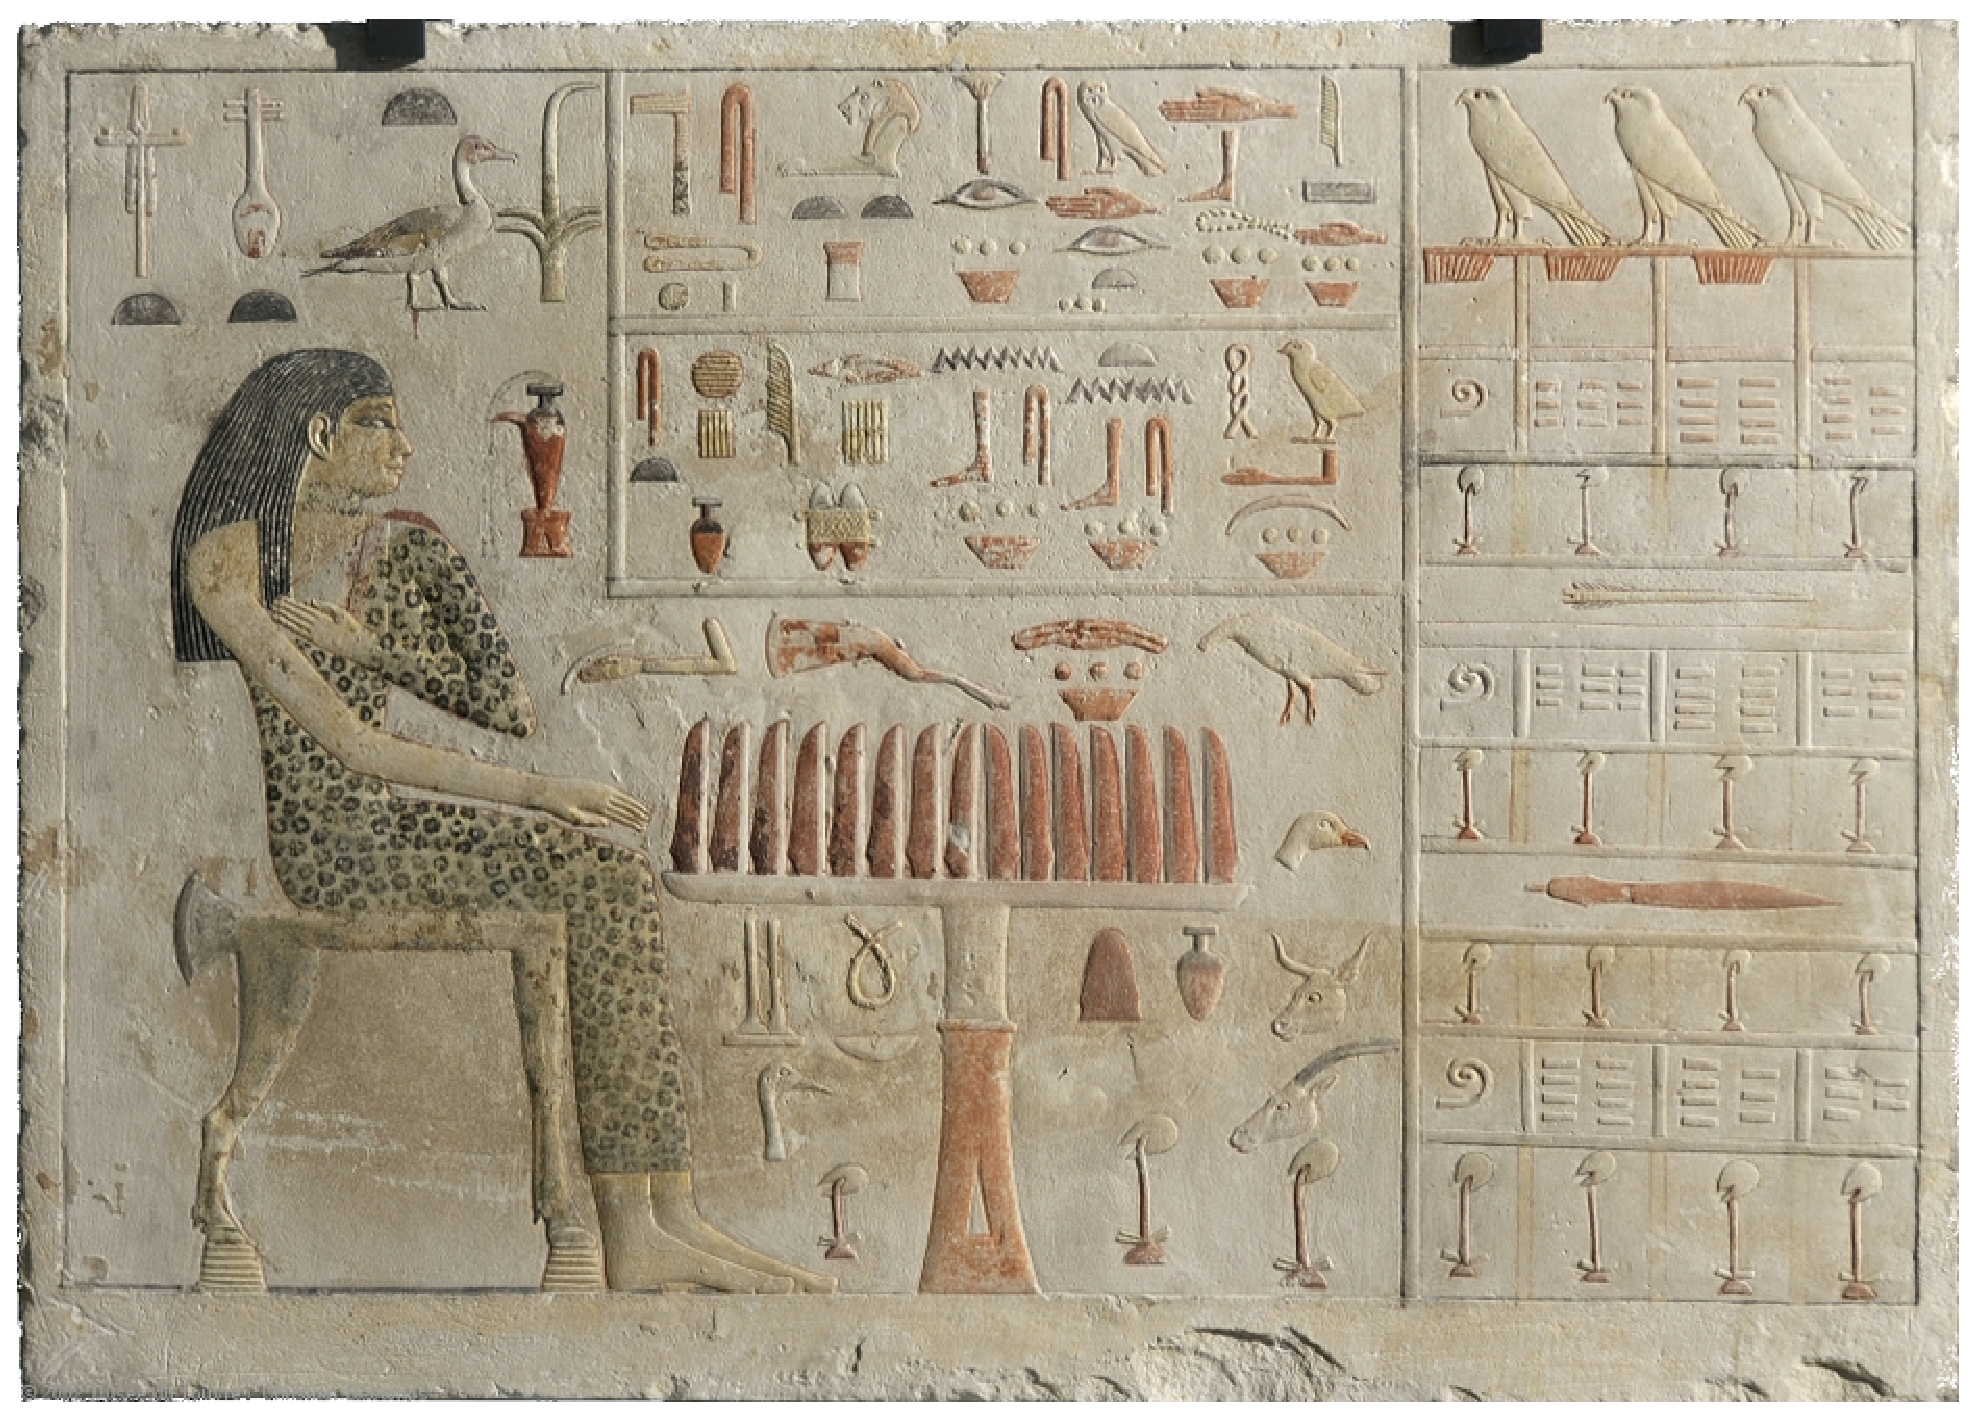
\includegraphics[height=6cm]{Nombres_et_calculs/Images/N1_intro_Nefertiabet}
   \caption{La princesse Néfertiabet devant son repas. Musée du Louvre, Christian Décamps}
\end{figure}

\vfill
\begin{prerequis}[Un peu d'histoire]
   Le système de numération que nous employons actuellement et qui nous semble si naturel est le fruit d'une longue évolution des concepts mathématiques. En effet, un nombre est une entité abstraite qui peut surprendre : on a déjà vu \textit{un} élève, \textit{un} animal donné, on sait ce qu'est \textit{un} jour de congé, mais qu'est-ce que \textit{un} ? C'est une entité qui, prise seule, n'a pas vraiment de sens. De nombreuses civilisations ont imaginé des systèmes de numération plus ou moins compliqués, plus ou moins pratiques : le plus ancien système semble avoir vu le jour en Mésopotamie dès le {\small IV}\up{e} siècle avant J.-C. Après avoir expérimenté des systèmes utilisant des bases et des principes différents, le système de numération positionnel de base dix est maintenant utilisé de manière universelle.
\end{prerequis}



\cours %%%%%%%%%%%%%%%%%%%%%%%%%
%%%%%%%%%%%%%%%%%%%%%%%%%%%%

%%%%%%%%%%%%%%%%%%%%%%%%%%%%
\section{Différents types de numération} %%%%%%%%

\begin{definition}[Numération]
   On appelle \textbf{numération}, tout code permettant de représenter un nombre.
\end{definition}

   \medskip
   
   Une numération peut être gestuelle, écrite ou orale et ne se limite pas à un ensemble de signes (le vocabulaire), elle fonctionne avec des règles d'agencement de ces signes (la grammaire). Il existe de nombreux systèmes de numération, chacun lié à une ou plusieurs grandes civilisations. \\
   Il existe trois familles principales de systèmes de numération : {\bf additif, hybride et positionnel}.
    
    
\subsection{Deux exemples de système additif : les égyptiens et les romains} %%%

   Pendant probablement plus de 3\,600 ans, les Égyptiens ont utilisé des hiéroglyphes pour écrire. La plus ancienne inscription a été découverte en 1992 et est datée d'environ $-3\,200$ av. J.-C. L'écriture hiéroglyphique a été déchiffrée à partir de 1821 par Jean-François {\bf Champollion} grâce à la pierre de Rosette.

   Dans cette numération, chaque symbole renvoie à une quantité toujours identique et ceci indépendamment de la position qu'il occupe dans l'écriture du nombre. Le nombre codé est obtenu par addition de toutes les quantités représentées par les différents chiffres. Les signes utilisés par ce système sont indiqués dans le tableau ci-dessous :

\begin{center}
{\hautab{2.2}
\begin{Ltableau}{1\linewidth}{4}{c|l|r|p{10.8cm}}
   \hline
   hiéroglyphe & nom & valeur & mnémonique \\
   \hline
   \parbox{6mm}{\Huge \textpmhg{\Hone}} & trait & 1 & un bâton représentant l'unité \\
   \hline
   \parbox{6mm}{\huge \textpmhg{\Hten}} & pont & 10 & l'anse d'un panier qui contient environ 10 objets \\
   \hline
   \parbox{6mm}{\huge \textpmhg{\Hhundred}} & escargot & 100 & un rouleau de papyrus car on peut y écrire environ 100 hiéroglyphes \\
   \hline
   \parbox{6mm}{\huge \textpmhg{\Hthousand}} & lotus & 1\,000 & une fleur de lotus car on les trouve par milliers\\
   \hline
   \parbox{6mm}{\huge \textpmhg{\HXthousand}} & index & 10\,000 & un doigt montrant le ciel étoilé car on y voit près de 10\,000 étoiles \\
   \hline
   \parbox{6mm}{\huge \textpmhg{\HCthousand}} & têtard & 100\,000 & un têtard car on en trouve environ 100\,000 après la ponte \\
   \hline
   \parbox{6mm}{\huge \textpmhg{\Hmillion}} & dieu & 1\,000\,000 & un dieu agenouillé supportant la voute céleste car le dieu est éternel et un million d'années c'est l'éternité (!) \\    
   \hline
\end{Ltableau}}
\end{center}

Pour écrire les nombres, on juxtapose simplement autant de signes élémentaires que nécessaire. Il s'agit d'un \textbf{système additif} utilisant les groupements-échanges par 10 : on ne trouve jamais, dans l'écriture finale d'un nombre, plus de neuf signes identiques.

\begin{exemple*1}
   \begin{enumerate}
      \item \quad {\huge \textpmhg{\Hten}\textpmhg{\Hone}\textpmhg{\Hone}} \; et \; {\huge \textpmhg{\Hone}\textpmhg{\Hone}\textpmhg{\Hten}} \; et \; {\huge \textpmhg{\Hone}\textpmhg{\Hten}\textpmhg{\Hone}} sont trois écritures différentes du nombre 12 ($10+1+1$).
      \item \quad {\large \textpmhg{\Hthousand}} \, {\huge \textpmhg{\Hten}\textpmhg{\Hten}\textpmhg{\Hten}\textpmhg{\Hten}\textpmhg{\Hten}\textpmhg{\Hten}\textpmhg{\Hten}\,\textpmhg{\Hone}\textpmhg{\Hone}\textpmhg{\Hone}\textpmhg{\Hone}\textpmhg{\Hone}\textpmhg{\Hone}} représente $1\times1\,000+7\times10+6\times1 =1\,076$. \\ [-9mm]
   \end{enumerate}
\end{exemple*1}


À l'heure actuelle, nous utilisons encore (un peu) le système romain, par exemple pour le nom des rois, l'écriture des siècles et les numérotations de chapitres. Les signes utilisés sont indiqués dans le tableau ci-dessous :

\begin{center}
{\renewcommand{\arraystretch}{2}
\begin{Ltableau}{1\linewidth}{3}{c|r|p{13.7cm}}
   \hline
   chiffre & valeur & provenance possible \\
   \hline
   $\cRm{1}$ & 1 & une marque verticale  \\
   \hline
   $\cRm{5}$ & 5 & représente la main ouverte \\
   \hline
   $\cRm{10}$ & 10 & réunion de deux mains ouvertes \\
   \hline
   $\cRm{50}$ & 50 & moitié inférieure de l'étoile à six branches, représentant cent. La lettre $\psi$ évoluera vers le $\cRm{50}$ \\
   \hline
   $\cRm{100}$ & 100 & $\cRm{10}$ et $\cRm{1}$ superposés (étoile à six branches), transformé en $\supset\!\!\!|\!\!\!\subset$, puis abrégé en $\cRm{100}$, initiale de \textit{centum} \\
   \hline
   $\cRm{500}$ & 500 & la moitié de 1\,000, écrit C\!\!D \\
   \hline
   $\cRm{1000}$ & 1\,000 & $\cRm{10}$ entouré, écrit comme phi $\phi$, devenu C\!\!D, et enfin confondu avec $\cRm{1000}$, initiale de \textit{milia} \\
   \hline
\end{Ltableau}}
\end{center}  
  
Au Moyen Âge où il est utilisé, ce système utilise le groupement par dix et un groupement auxiliaires par cinq. \\
Il s'agit d'un système \textbf{additif}, mais aussi \textbf{soustractif} permettent des écritures plus courtes.

\begin{documentation}[Numération romaine]
\begin{itemize}
   \item Principe additif : tout signe placé à  la droite d'un autre signe représentant une valeur supérieure ou égale à la sienne s'ajoute à celui-ci.
   \item Principe soustractif : tout signe placé à la gauche d'un autre signe représentant une valeur supérieure à la sienne doit être soustrait du nombre indiqué à droite. \\
      Seuls les signes $\cRm{1}, \cRm{10}$ et $\cRm{100}$ peuvent être soustraits, et ce seulement pour des valeurs 10 fois supérieures au maximum.
   \item La même lettre ne peut pas être employée quatre fois consécutivement sauf pour le signe représentant 1000 : $\cRm{1000}$.
   \item Les valeurs sont groupées en ordre décroissant, sauf pour les valeurs à retrancher.
\end{itemize}
\ \\ [-13mm]
\end{documentation} 
   
\begin{exemple*1}   
   \begin{enumerate}
      \item Procédé additif : $\cRm{2015}$ représente $1\,000+1\,000+10+5 =2\,015$.

      \item Procédé soustractif : $\cRm{100}\cRm{1000}$ représente $1\,000-100 =900$.
      \item Combinaison : $\cRm{699}$ représente $500+100+(100-10)+(10-1)=699$.
      \item \attention 999 n'est pas représenté par {\small IM} mais par $\cRm{999}$  car on ne peut pas ôter 1 de 1\,000 !
   \end{enumerate}   
\end{exemple*1}  
  
\bigskip
 
   Le système est vite limité pour écrire des grands nombres (supérieurs à 4\,999). Plus tard, les romains ajouteront une barre au dessus des signes multipliant par 1\,000 leur valeur initiale.


\subsection{Un exemple de sytème hybride : les chinois} %%%

   Dès le début de notre ère, les chinois disposent du système de notation de nombres qu'ils utilisent encore aujourd'hui. Ils ont neuf caractères pour les unités de un à neuf et un caractère pour chacune des puissances de dix. Ils utilisent des classes d'amplitude 1\,000. C'est un système sans irrégularités, contrairement au nôtre !
   
\begin{exemple*1}
   En chinois, le nombre 71 755 875 s'écrit 7175 5875 et se lit : \\
   \og sept mille un cent sept dix cinq dix mille - cinq mille huit cent sept dix cinq \fg. 
\end{exemple*1}

\bigskip

C'est un \textbf{système hybride} de base 10 dont les nombres sont représentés par addition de multiples de puissances de la base. Les signes chinois sont ceux du tableau ci-dessous et les nombres s'écrivent de haut en bas.

\begin{center}
{\renewcommand{\arraystretch}{1.5}
\begin{Ctableau}{1\linewidth}{14}{c}
   \hline
   signe & 
\includegraphics[width=5mm]{Nombres_et_calculs/Images/N1_chinois1} & 
\includegraphics[width=5mm]{Nombres_et_calculs/Images/N1_chinois2} & 
\includegraphics[width=5mm]{Nombres_et_calculs/Images/N1_chinois3} & 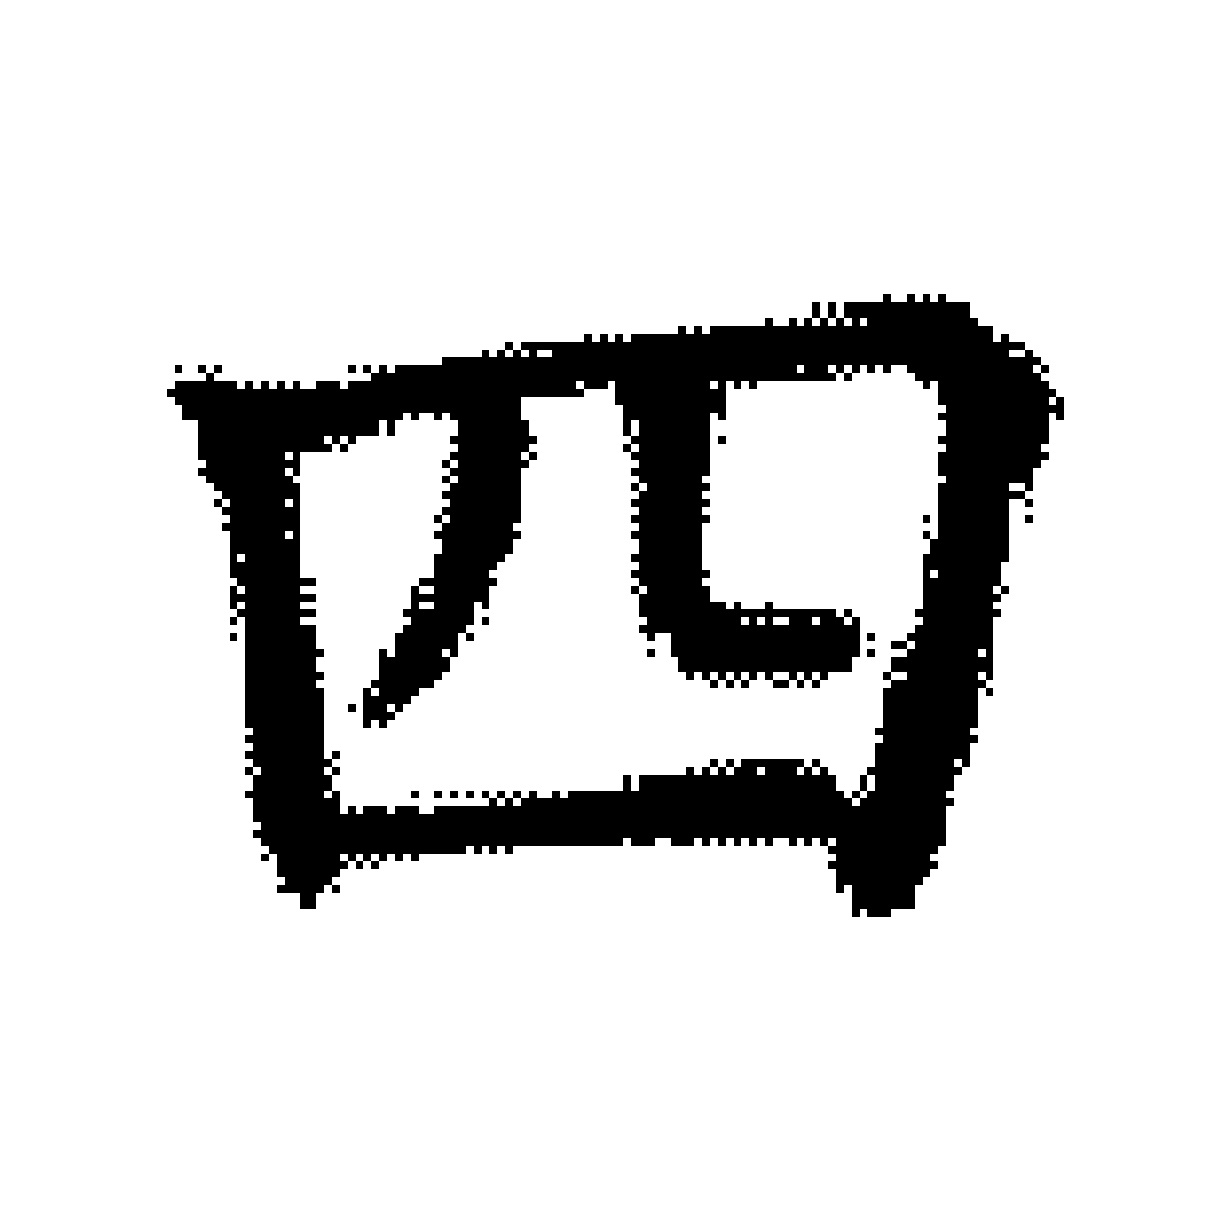
\includegraphics[width=5mm]{Nombres_et_calculs/Images/N1_chinois4} & 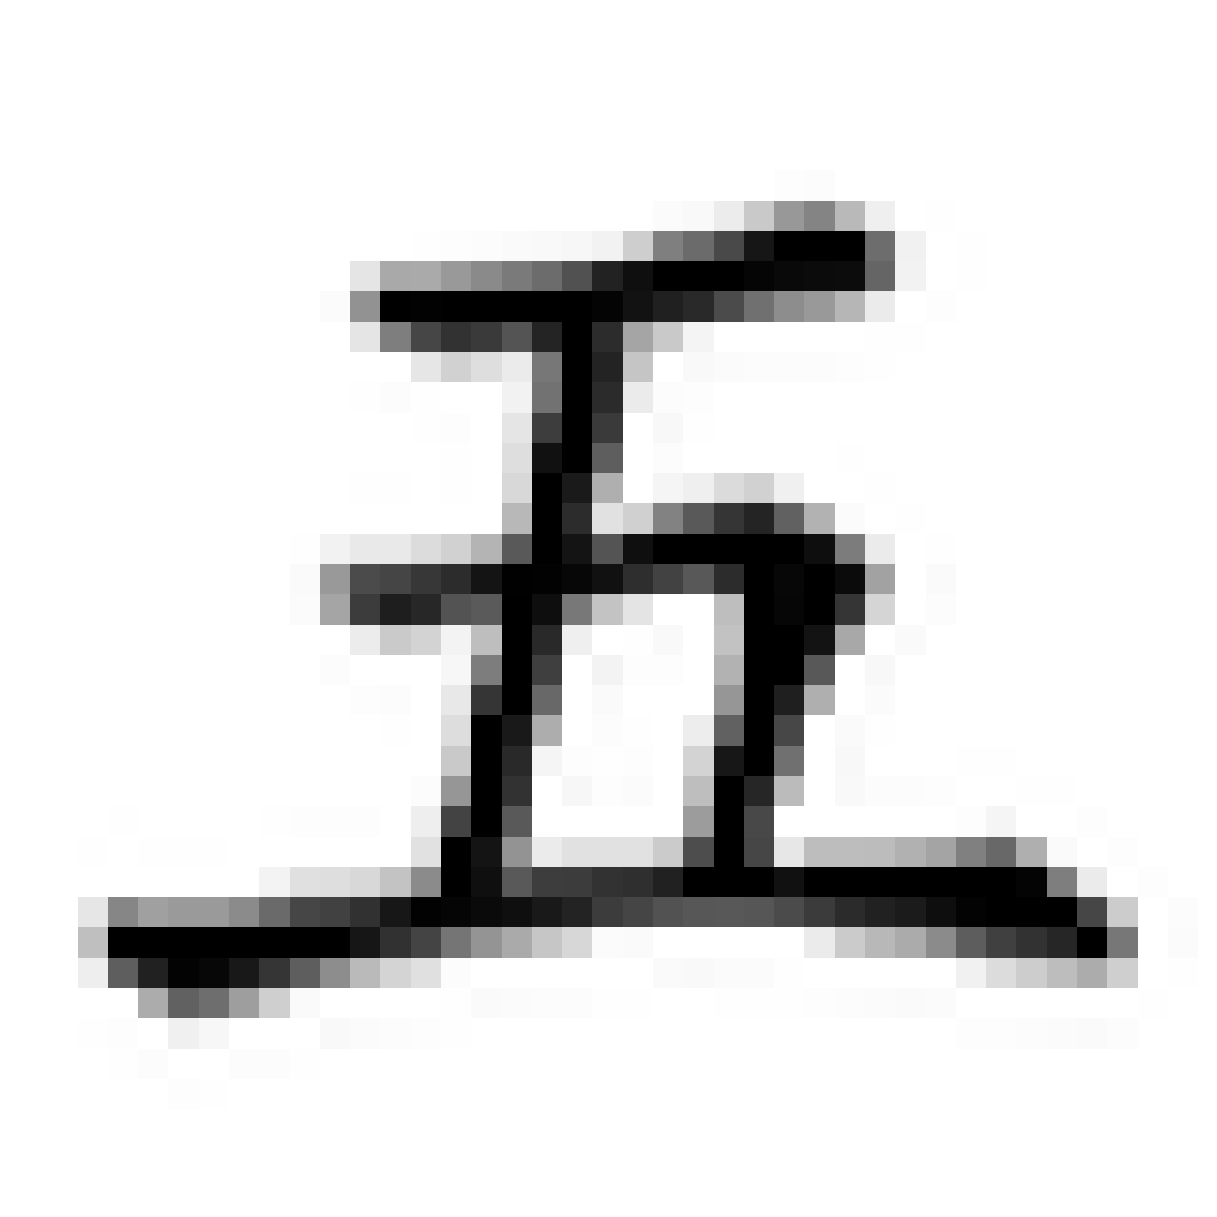
\includegraphics[width=5mm]{Nombres_et_calculs/Images/N1_chinois5} & 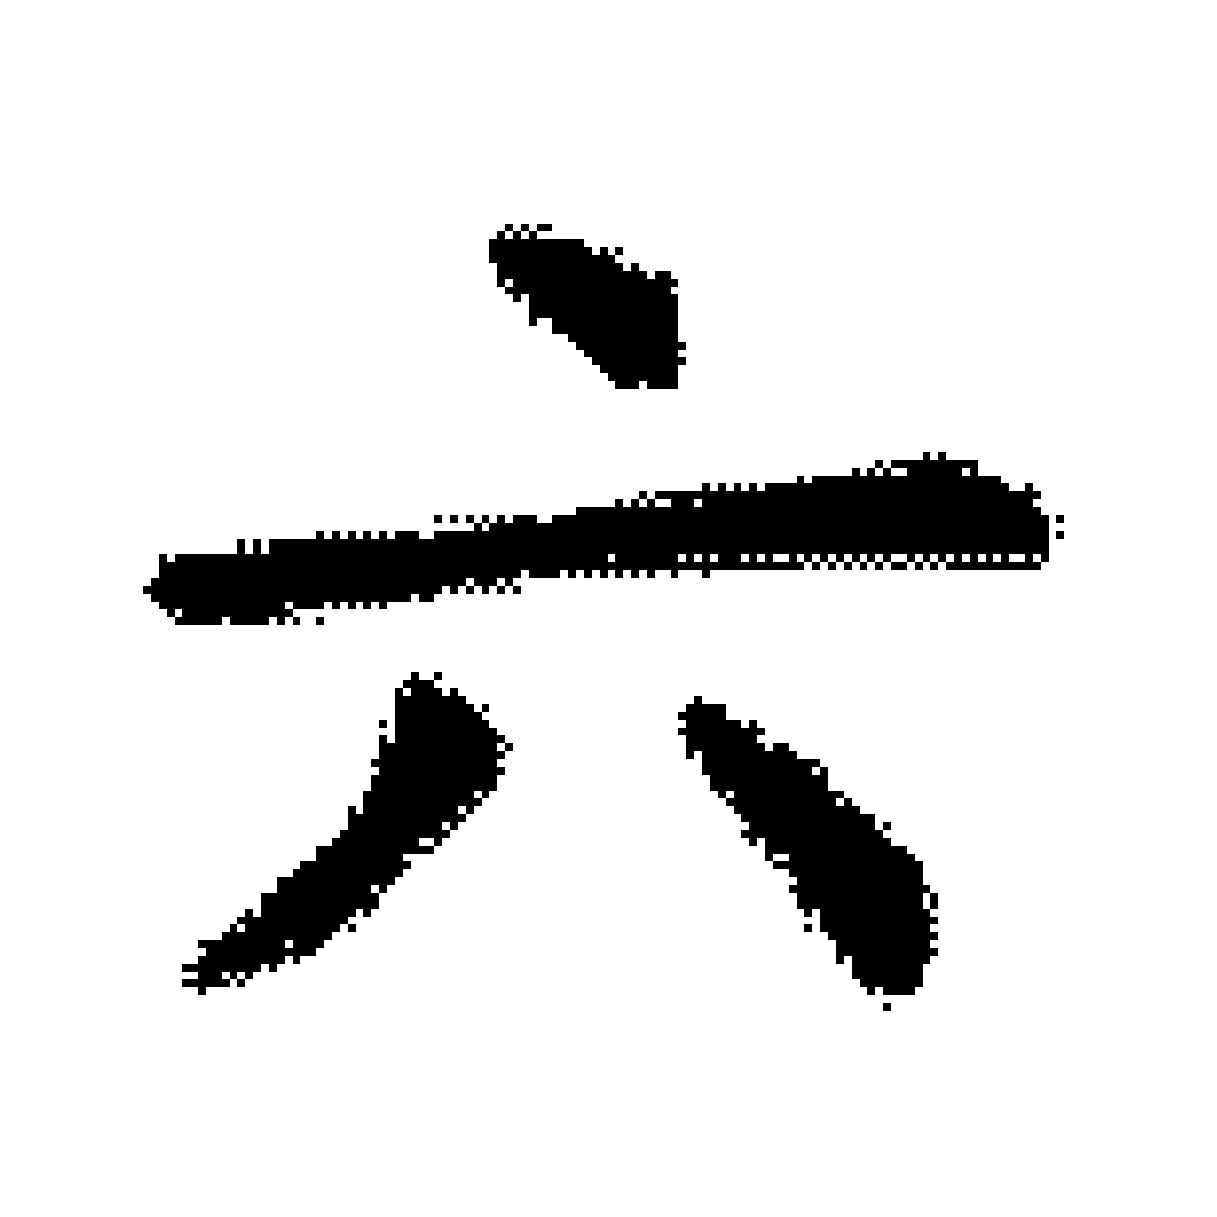
\includegraphics[width=5mm]{Nombres_et_calculs/Images/N1_chinois6} & 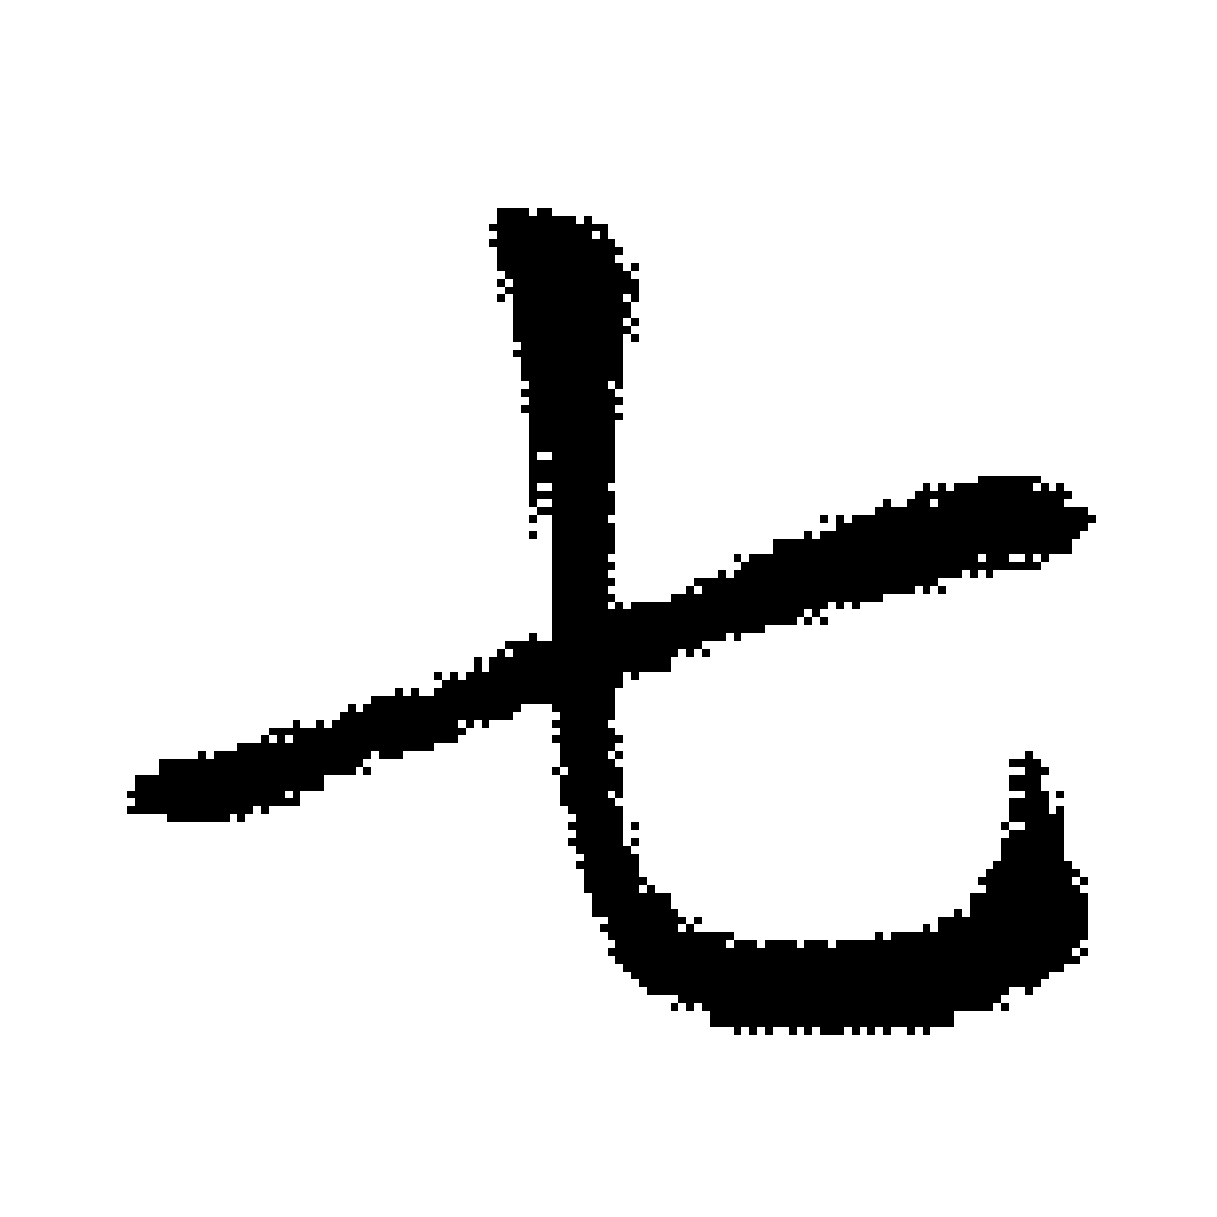
\includegraphics[width=5mm]{Nombres_et_calculs/Images/N1_chinois7} & 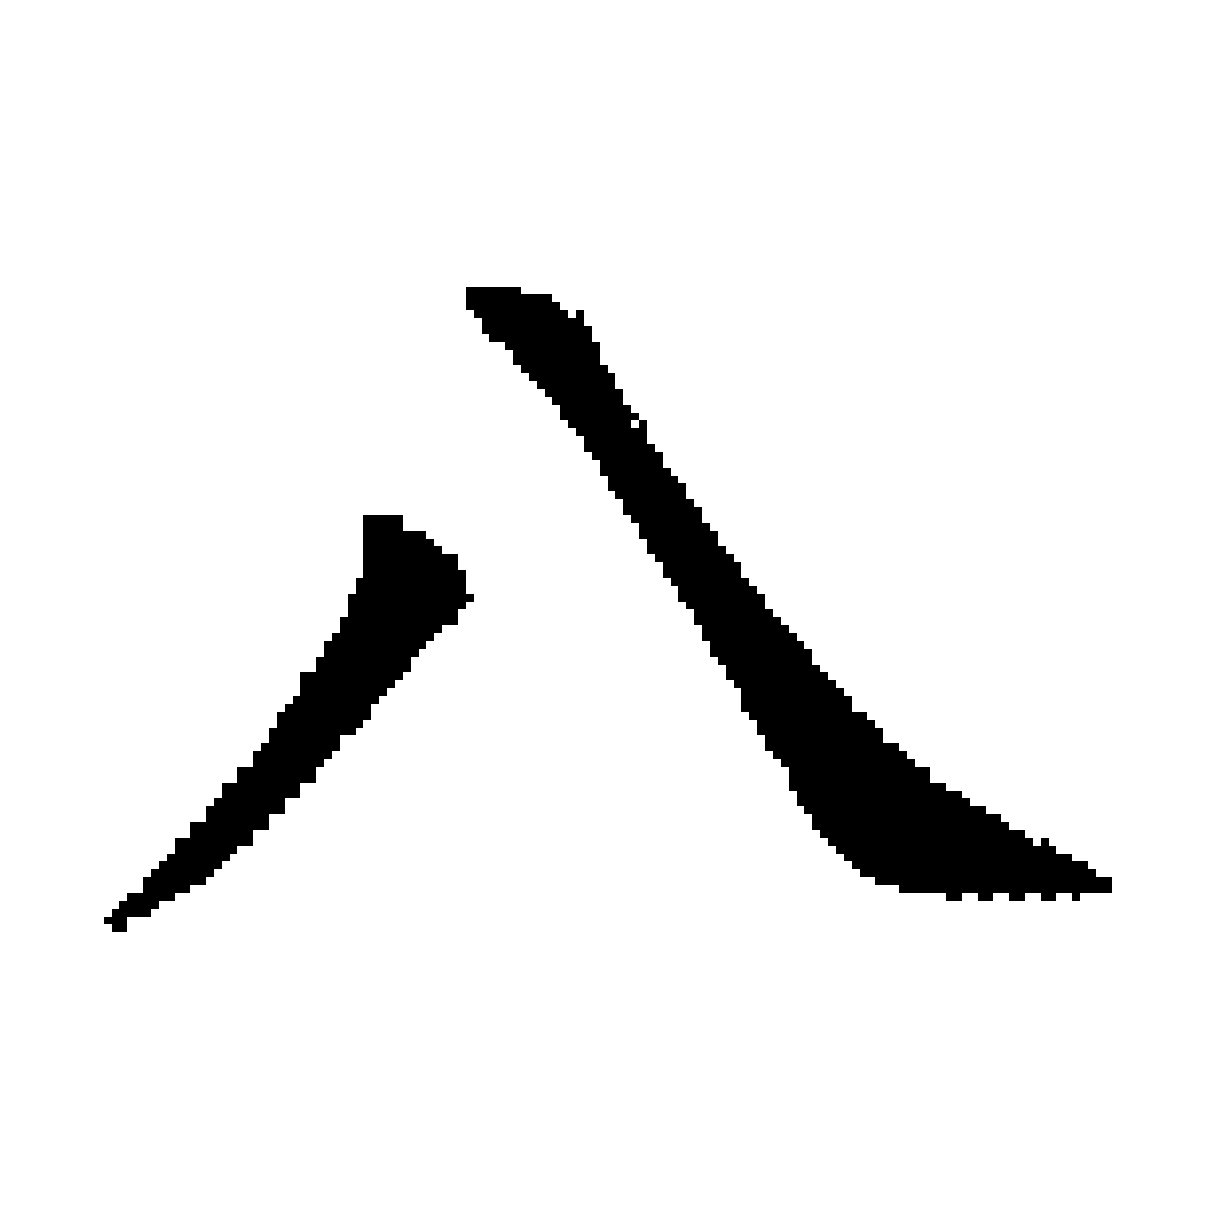
\includegraphics[width=5mm]{Nombres_et_calculs/Images/N1_chinois8} & 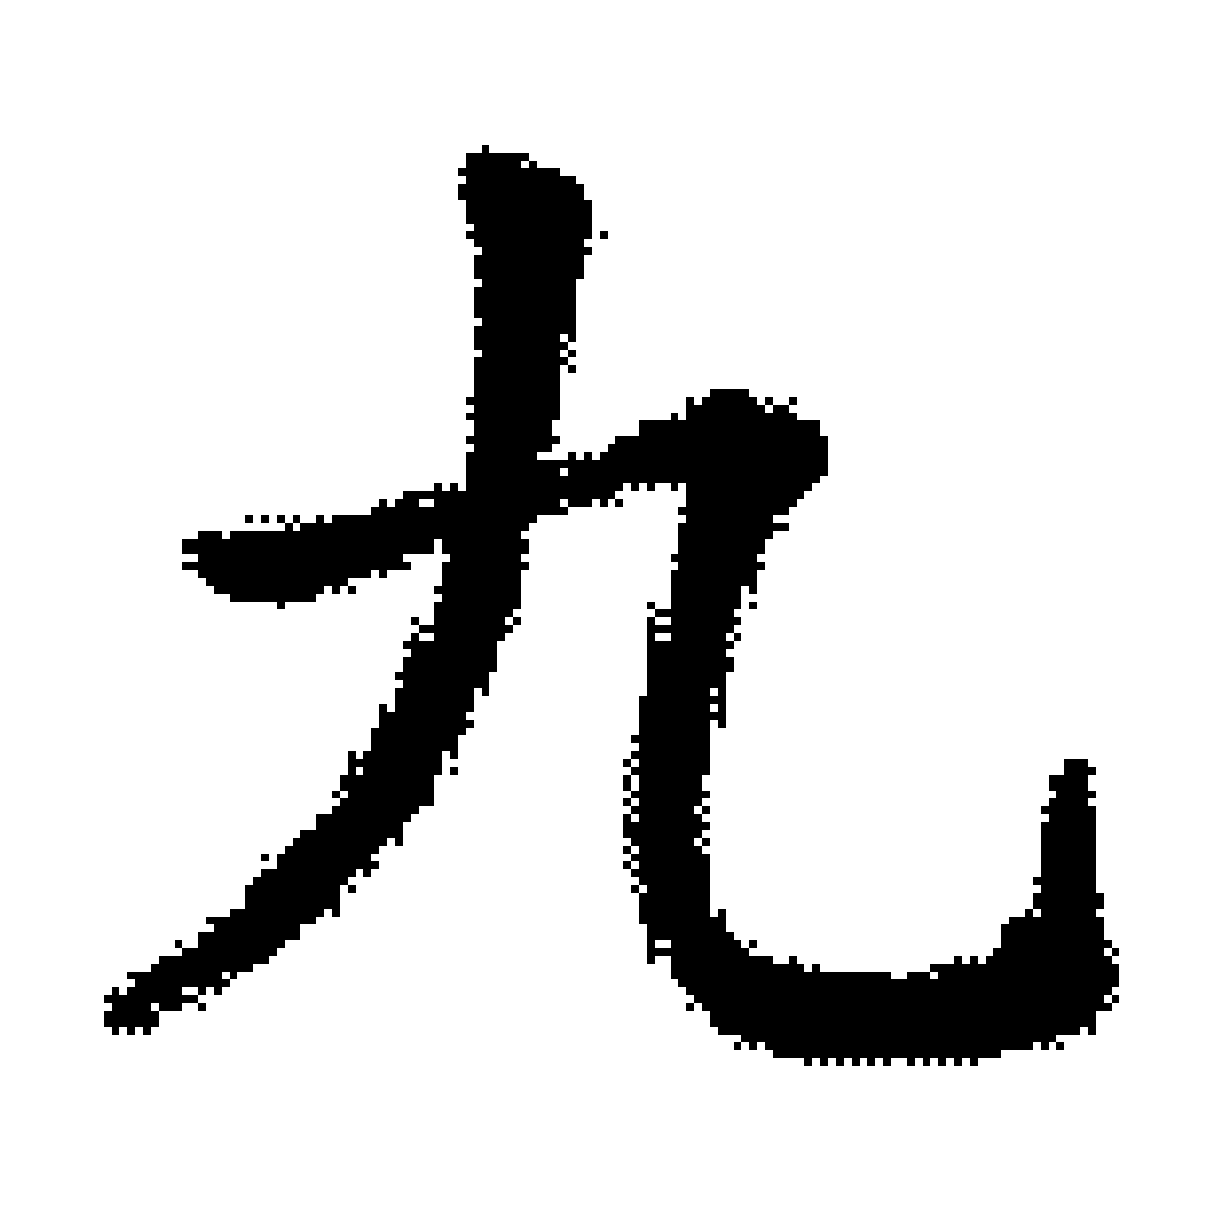
\includegraphics[width=5mm]{Nombres_et_calculs/Images/N1_chinois9} & 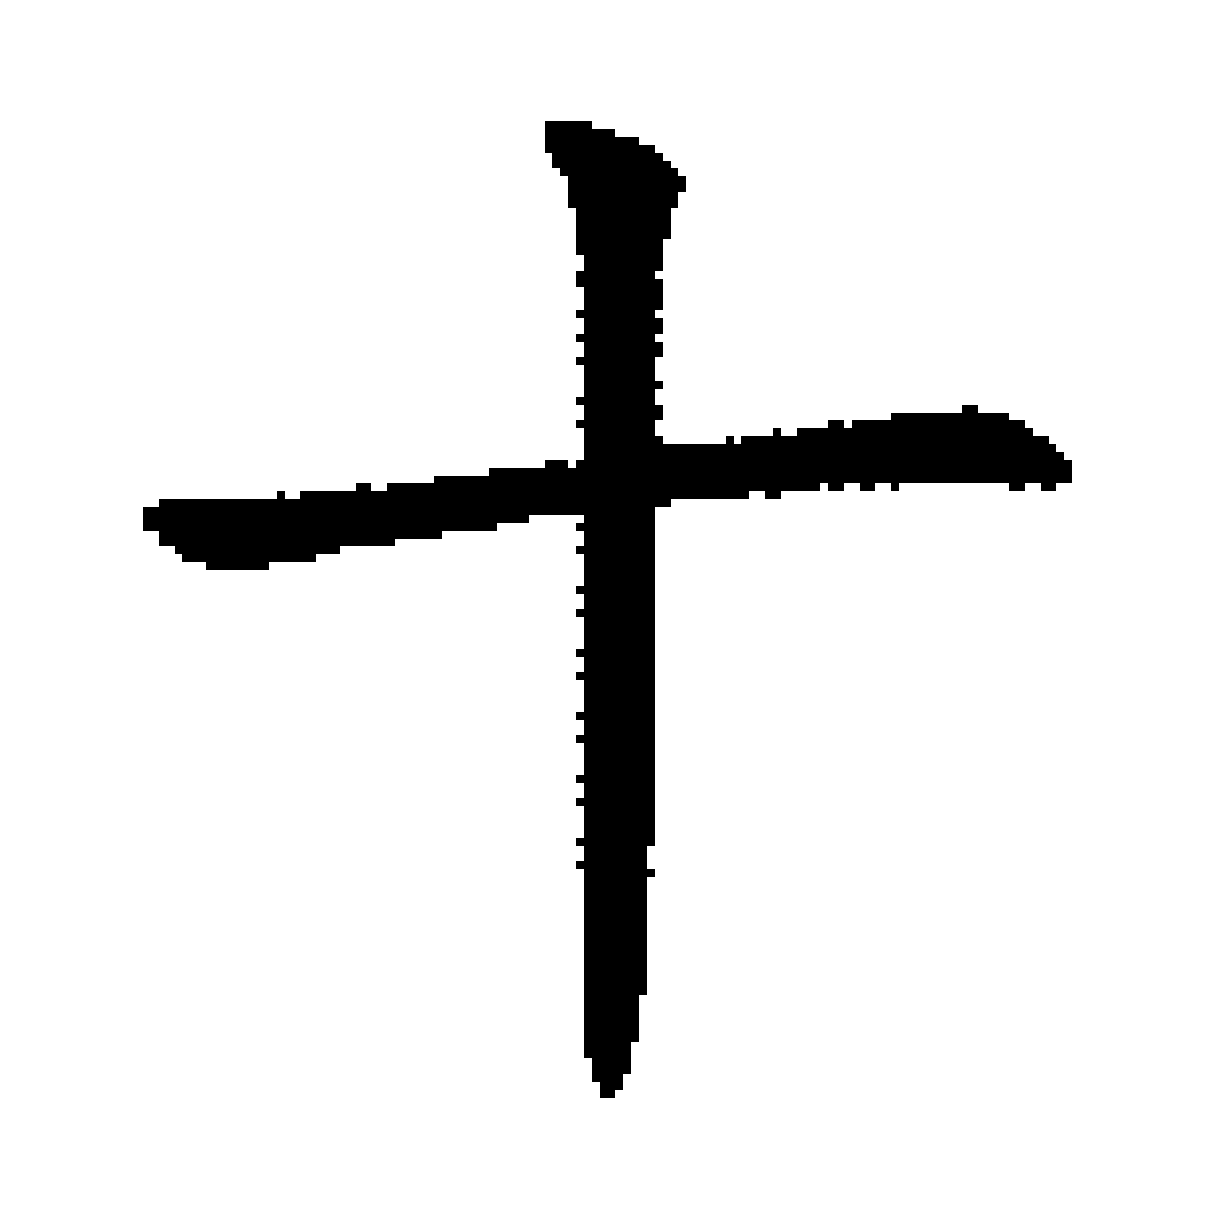
\includegraphics[width=5mm]{Nombres_et_calculs/Images/N1_chinois10} & 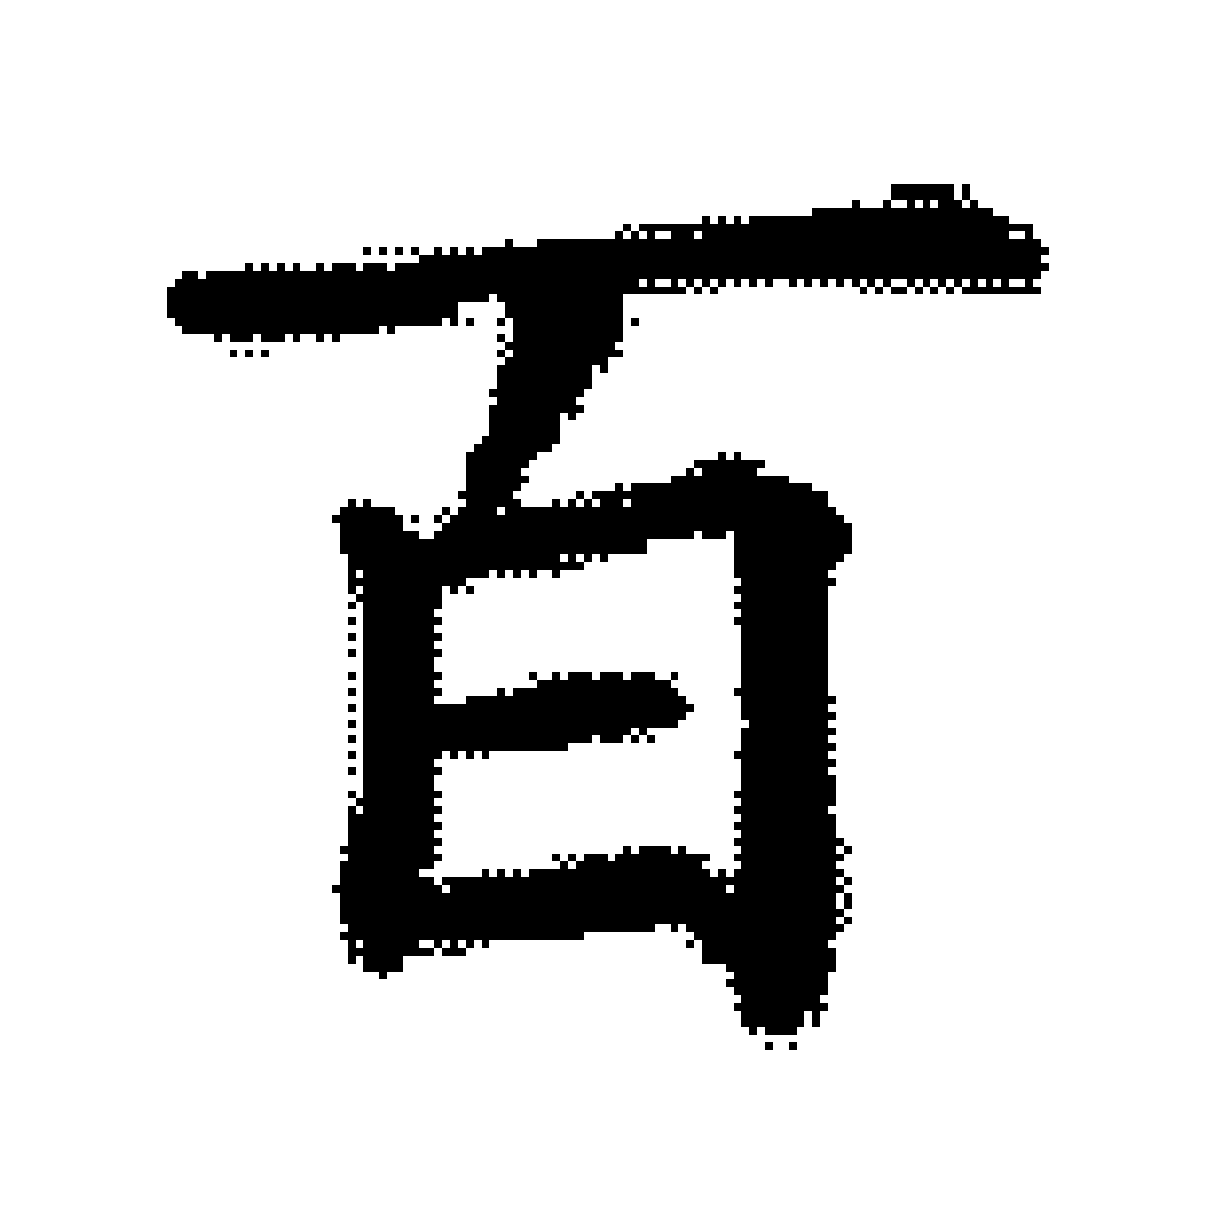
\includegraphics[width=5mm]{Nombres_et_calculs/Images/N1_chinois100} & 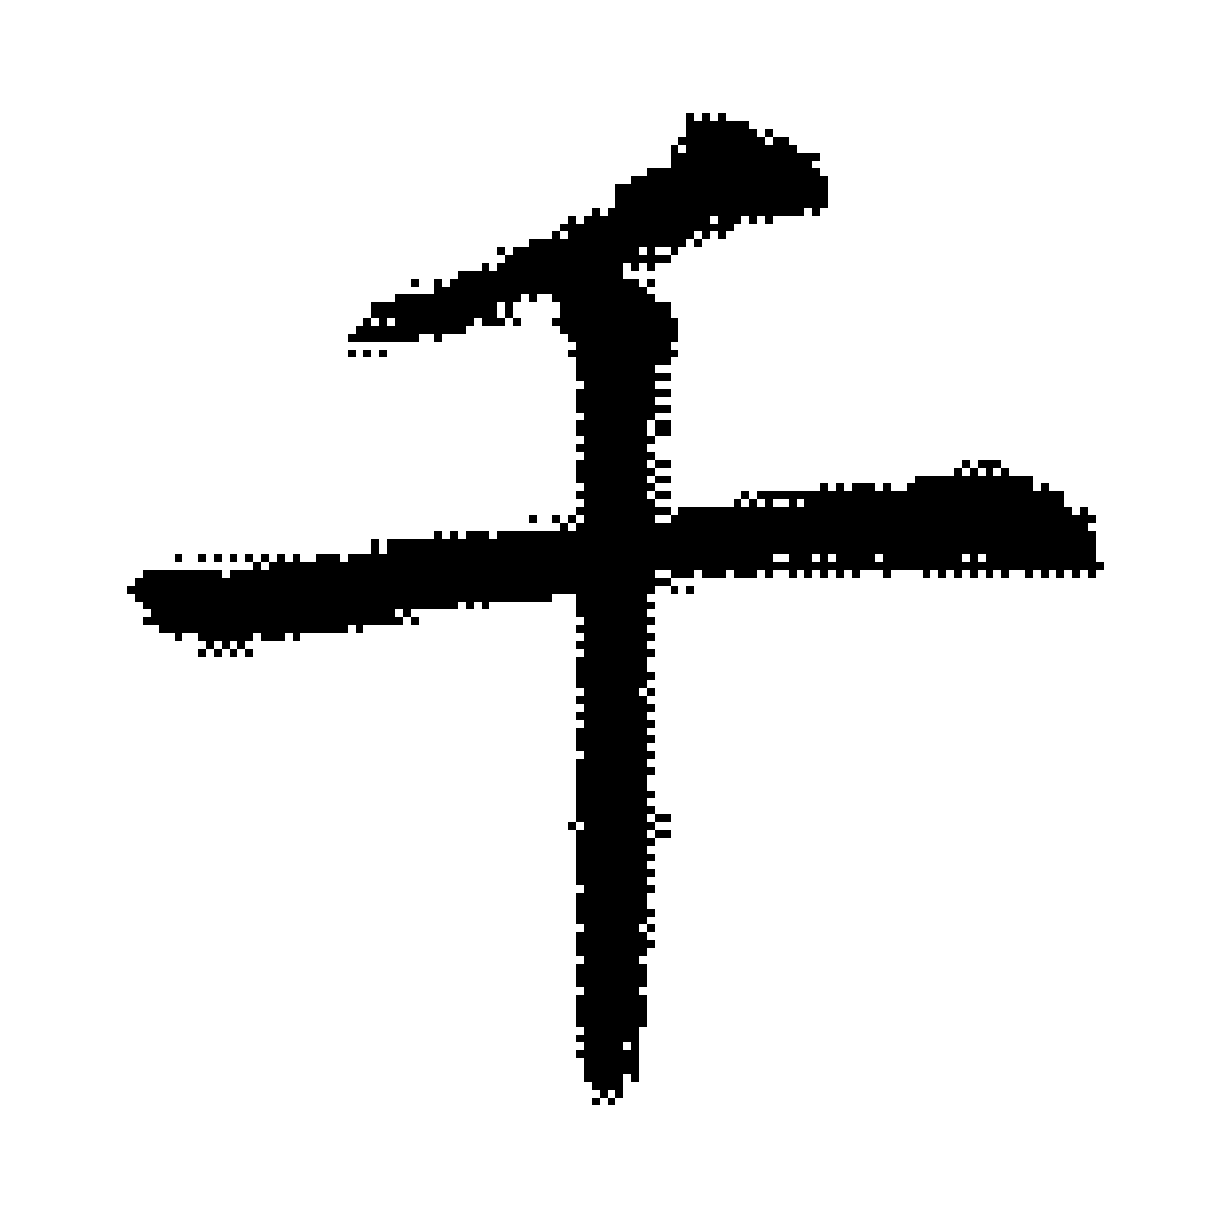
\includegraphics[width=5mm]{Nombres_et_calculs/Images/N1_chinois1000} & 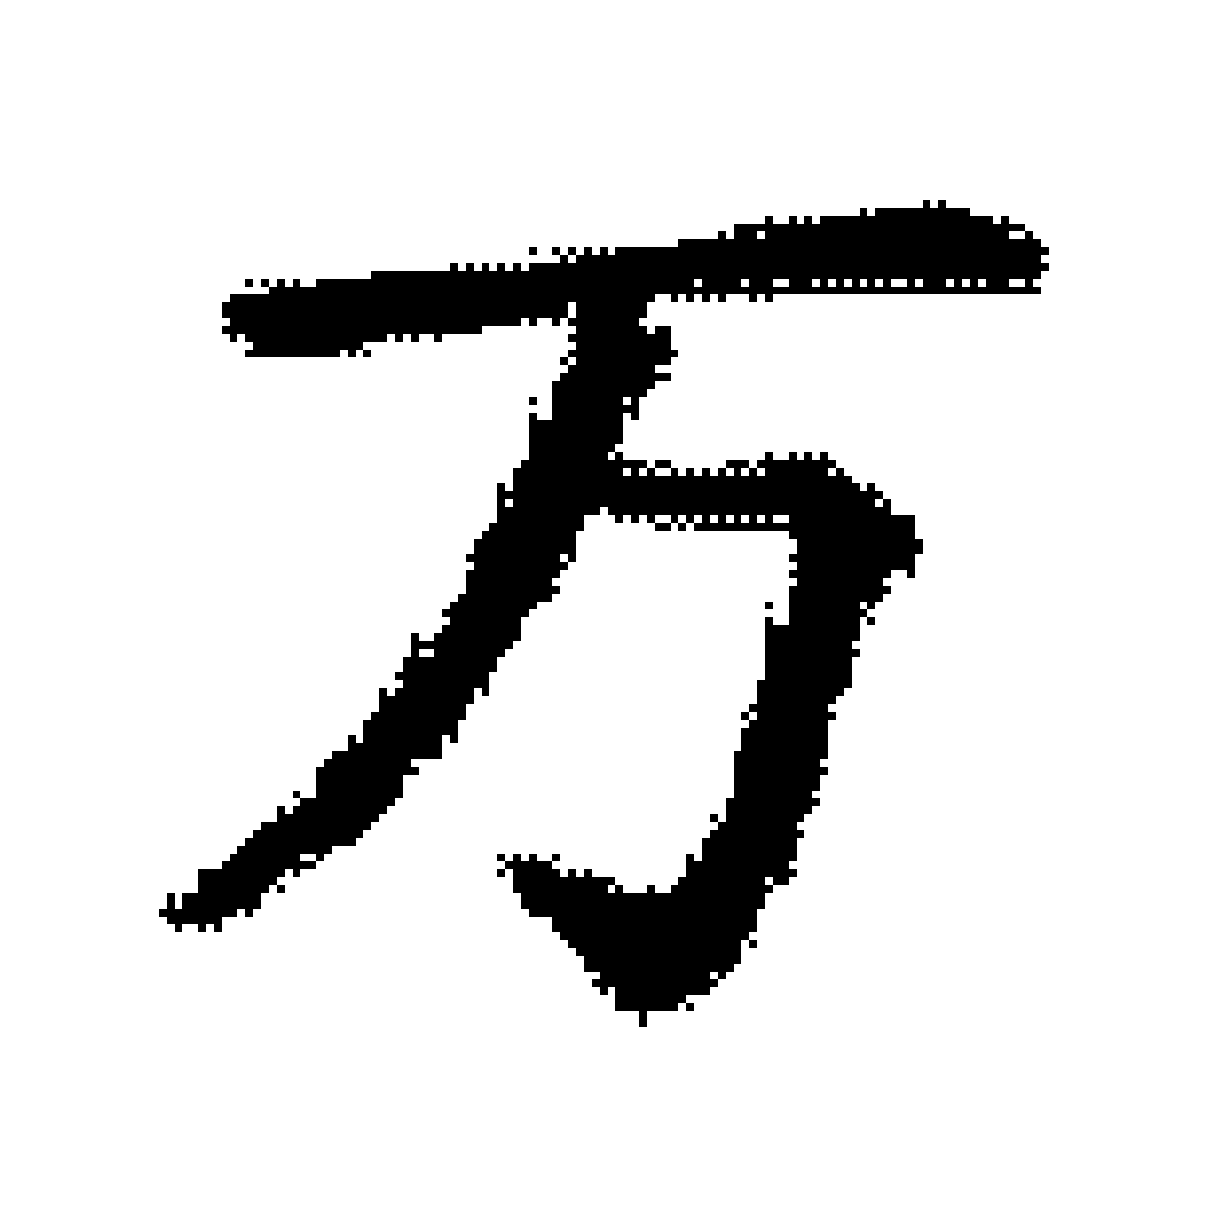
\includegraphics[width=5mm]{Nombres_et_calculs/Images/N1_chinois10000} \\ 
   \hline
   valeur & 1 & 2 & 3 & 4 & 5 & 6 &7 & 8 & 9 &10 & 100 & 1\,000 & 10\,000 \\
   \hline 
\end{Ctableau}}
\end{center}

\smallskip

\begin{exemple*1}
   {\renewcommand{\arraystretch}{0.5}
   28 s'écrit \begin{tabular}{c}
      
\includegraphics[width=5mm]{Nombres_et_calculs/Images/N1_chinois2} \\
      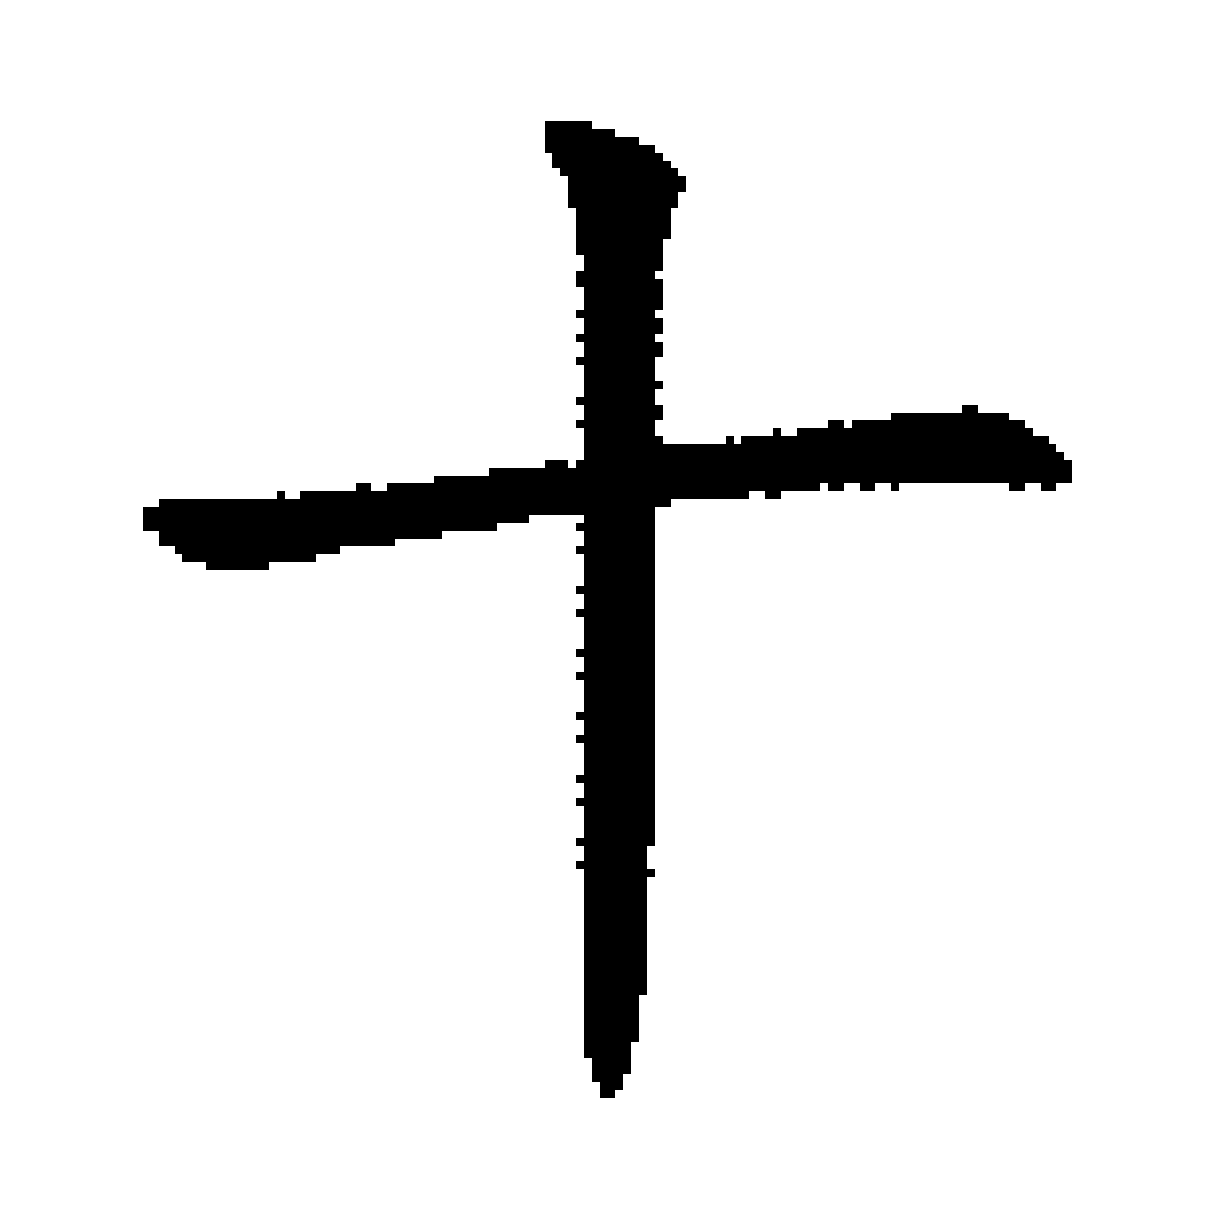
\includegraphics[width=5mm]{Nombres_et_calculs/Images/N1_chinois10} \\
      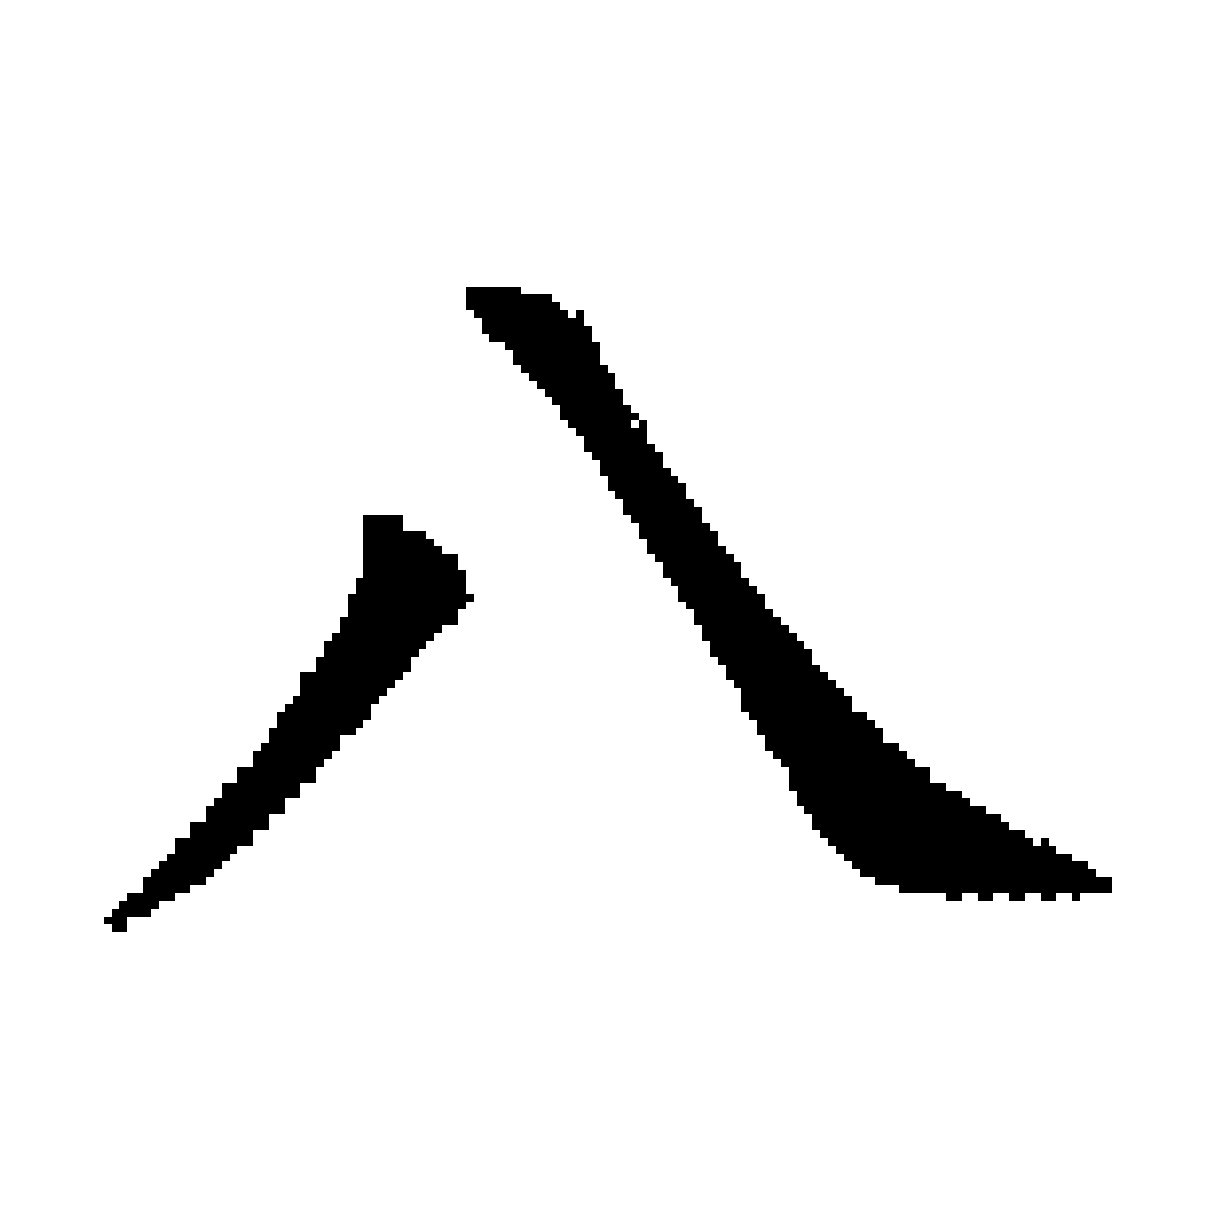
\includegraphics[width=5mm]{Nombres_et_calculs/Images/N1_chinois8} \\
   \end{tabular} et \numprint{4092} s'écrit
   \begin{tabular}{c}
      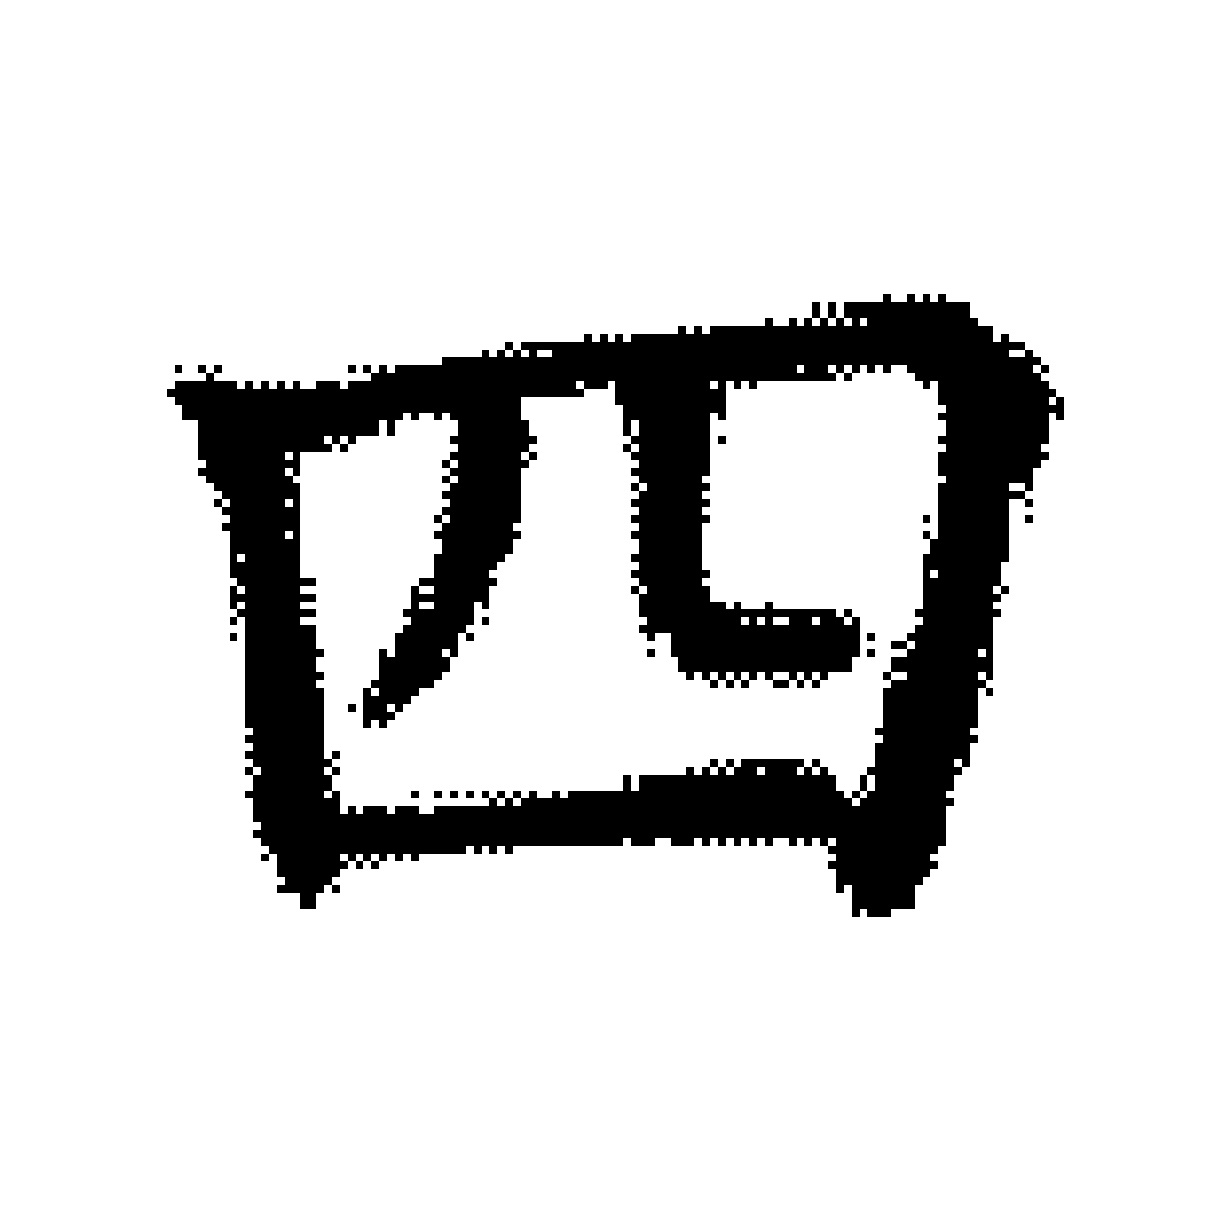
\includegraphics[width=5mm]{Nombres_et_calculs/Images/N1_chinois4} \\
      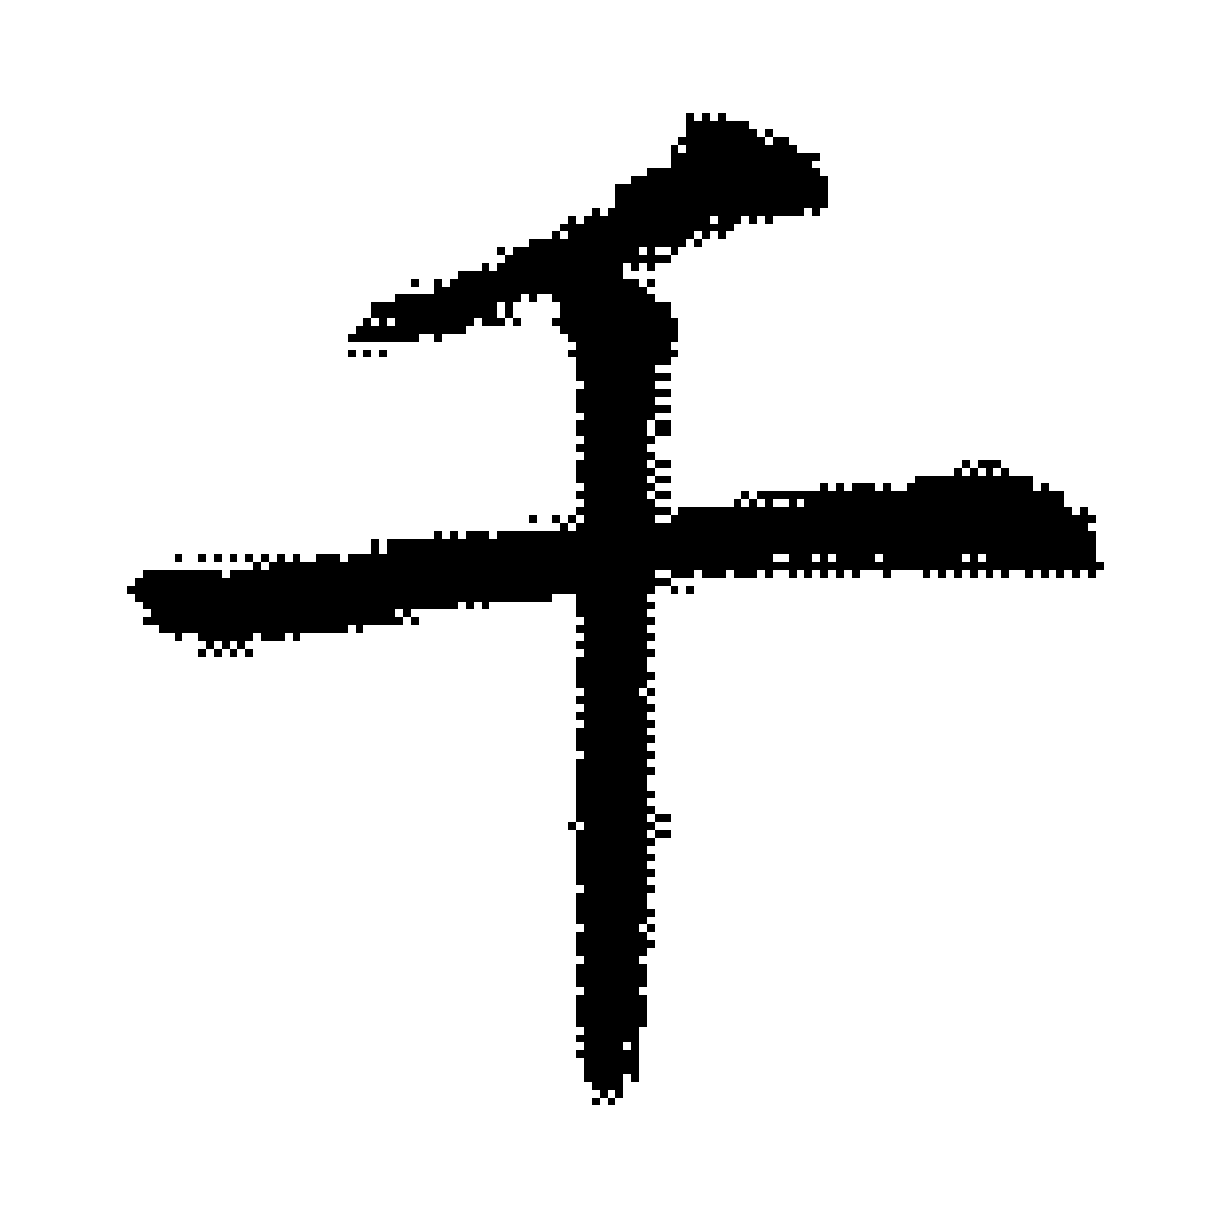
\includegraphics[width=5mm]{Nombres_et_calculs/Images/N1_chinois1000} \\
      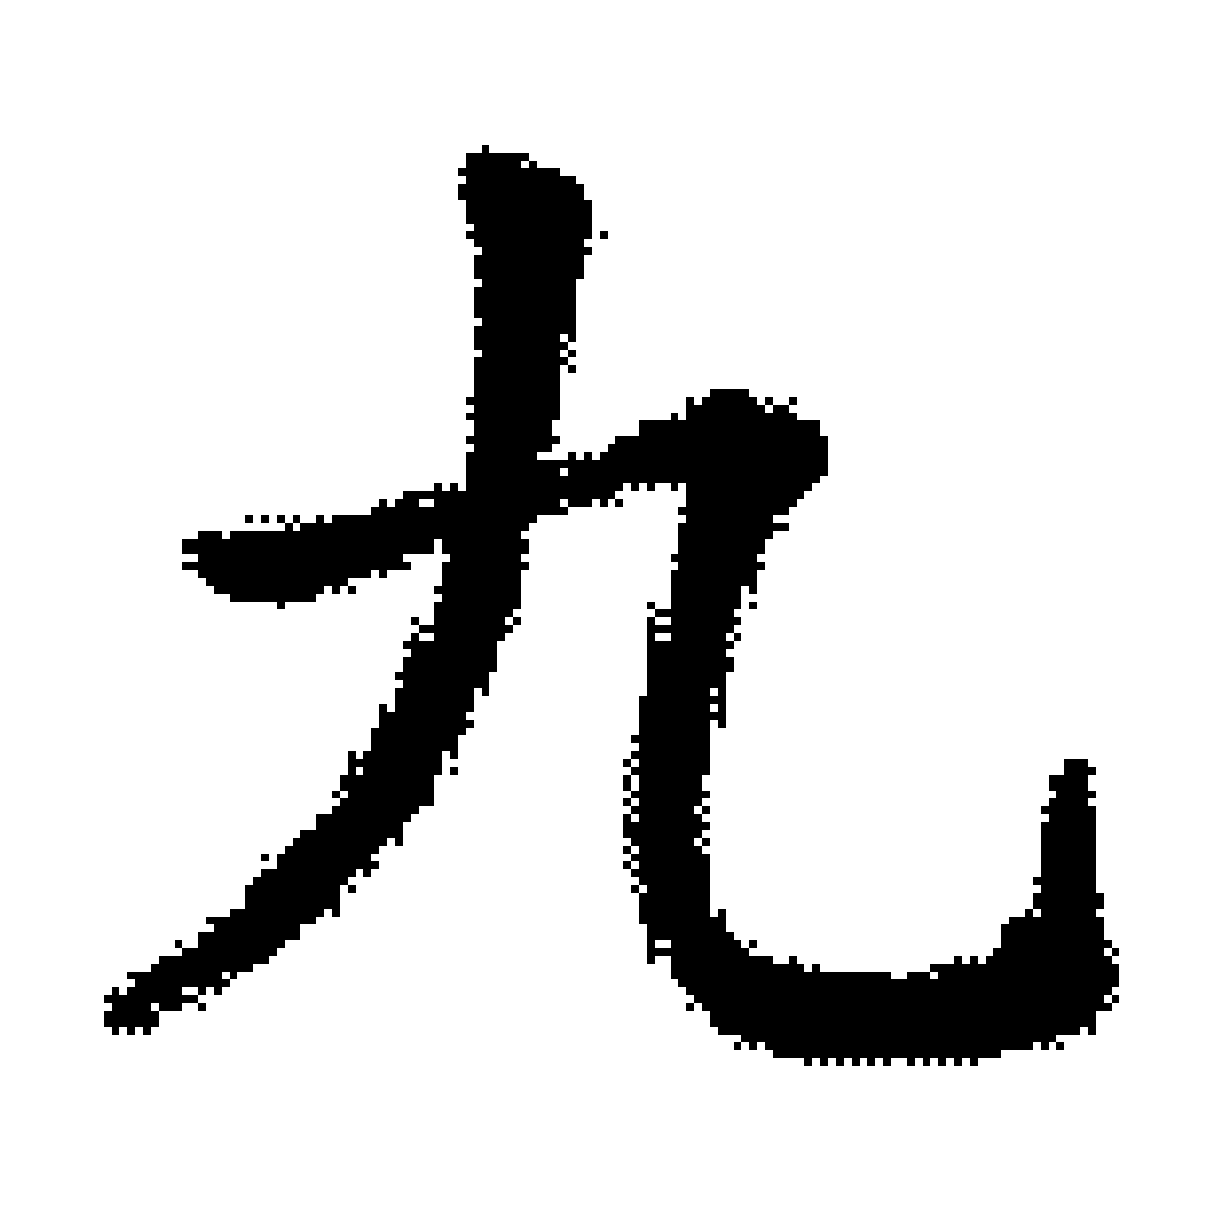
\includegraphics[width=5mm]{Nombres_et_calculs/Images/N1_chinois9} \\
      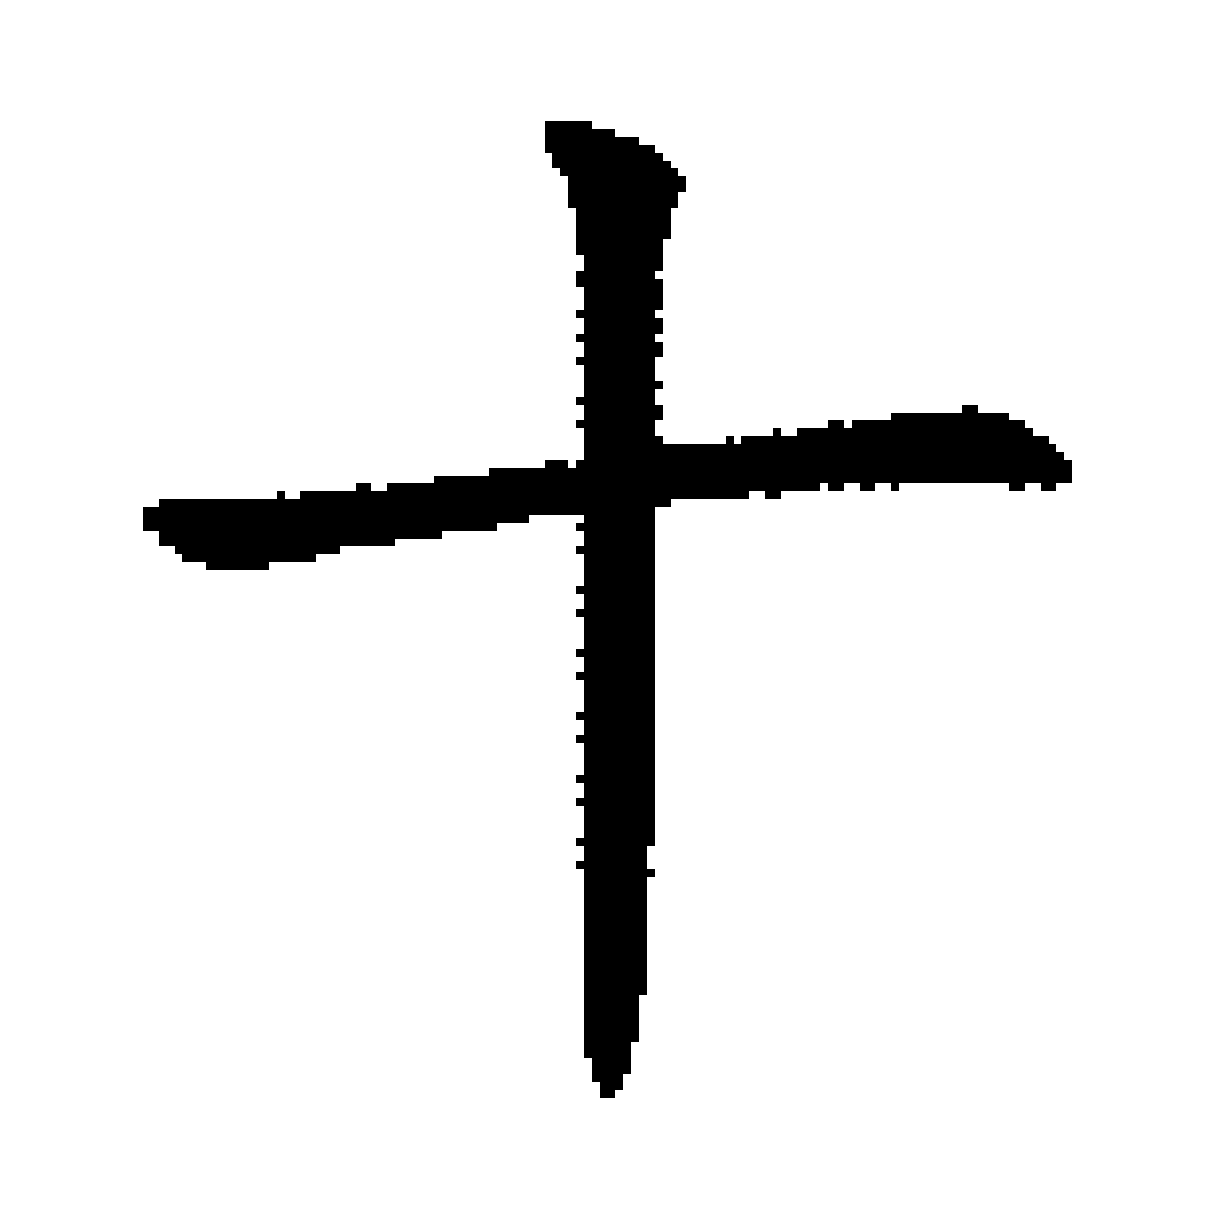
\includegraphics[width=5mm]{Nombres_et_calculs/Images/N1_chinois10} \\
      
\includegraphics[width=5mm]{Nombres_et_calculs/Images/N1_chinois2} \\
   \end{tabular}}
\end{exemple*1}


\subsection{Un exemple de système positionnel : le babyloniens} %%%

   Les Babyloniens ont utilisé de nombreuses bases différentes. Nous nous intéresserons ici à un système très élaboré à base 60 (voir \S 2.), qui leur a servi pour les tables astronomiques. Notre propre calcul du temps en heures, minutes, secondes, et notre calcul des angles en degrés sont des vestiges de ce système vieux de quatre mille ans.\\
   Le système babylonien est un \textbf{système positionnel} de base 60 (système sexagésimal) et de base secondaire 10, et il est additif pour les nombres inférieurs à 60. Chacun des chiffres est écrit au moyen de seulement deux signes : le clou \textcugar{g} valant 1 et le chevron \textcugar{`} valant 10. Le tableau suivant montre comment étaient écrits quelques chiffres.

\begin{center}
{\renewcommand{\arraystretch}{1.5}
\begin{Ctableau}{0.82\linewidth}{10}{C{1}|C{0.8}|C{0.8}|C{0.8}|C{0.8}|C{0.8}|C{0.8}|C{0.8}|C{0.8}|C{2}}
   \hline
   signe & \textcugar{g} & \textcugar{g}\textcugar{g} & \textcugar{g}\textcugar{g}\textcugar{g} & \ldots & \textcugar{`} & \textcugar{`}\textcugar{g} &  \textcugar{`}\textcugar{g}\textcugar{g} &  \ldots  & \textcugar{`}\textcugar{`}\textcugar{`}\textcugar{`}\textcugar{`}\textcugar{h}\textcugar{h}\textcugar{h} \\
   \hline
   valeur & 1 & 2 & 3 & \ldots & 10 & 11&12 &  \ldots & 59 \\
   \hline
\end{Ctableau}}
\end{center}

\begin{exemple*1}
\setlength{\tabcolsep}{0pt}
Pour écrire \numprint{10000} en babylonien, on effectue les divisions euclidiennes par 60 : $\qquad \begin{tabular}[b]{*{5}{C{0.3}}|*{3}{C{0.3}}} 1 & 0 & 0 & 0 & 0 & 6 & 0 & \\ \cline{6-8} & & & \textcolor{A1}{4} & \textcolor{A1}{0} &1 & 6 & 6 \\ \end{tabular} \qquad\opidiv[remainderstyle=\textcolor{A1}]{166}{60} \qquad\opidiv[remainderstyle=\textcolor{A1}]{2}{60}$ \\  
   Puis on écrit de droite à gauche les restes successifs des divisions : \textcolor{A1}{2\,46\,40}, que l'on \og transcrit \fg{} en babylonien : \textcugar{g}\textcugar{g} \, \textcugar{`}\textcugar{`}\textcugar{`}\textcugar{`}\textcugar{g}\textcugar{g}\textcugar{g}\textcugar{g}\textcugar{g}\textcugar{g}\, \textcugar{`}\textcugar{`}\textcugar{`}\textcugar{`} \\
   On peut également décomposer \numprint{10000} selon les puissances décroissantes de 60 : \\
   $10\,000=\textcolor{A1}{2}\times 60^2+\textcolor{A1}{46}\times 60+\textcolor{A1}{40}$.
\end{exemple*1}

\begin{remarque}
   dans un premier temps, les mésopotamiens ne possédaient pas le zéro, ce nombre pouvait donc aussi représenter $2\times60^{\textcolor{A1}{3}}+46\times 60+40=434\;800$. C'était alors le contexte qui renseignait l'ordre du nombre !
\end{remarque}



%%%%%%%%%%%%%%%%%%%%%%%%%%
\section{Les bases}

\subsection{Notre système de numération} %%%

   La notation positionnelle est un procédé d'écriture des nombres, dans lequel chaque position d'un chiffre ou symbole est reliée à la position voisine par un multiplicateur, appelé base du système de numération. Chaque position peut être renseignée par un symbole (notation sans base auxiliaire) ou par un nombre fini de symboles (notation avec base auxiliaire). 
   
Notre système de numération est un système positionnel de base dix sans  base auxiliaire et il est composé de dix chiffres indo-arabes (chiffres venus de l'Inde, mais utilisés et dispersés par les arabes).
      
\begin{exemple*1}
   \begin{enumerate}
      \item Dans l'écriture de 37, le chiffre 3 correspond à la quantité trente ;
      \item dans l'écriture de 73, le chiffre 3 correspond à la quantité trois ;

      \item dans l'écriture de 307, le chiffre 3 correspond à la quantité trois cents. Le 0 exprime l'absence de dizaine.
   \end{enumerate}
\end{exemple*1}
   
\begin{methode}[Notation \og usuelle \fg{} des nombres en base 10]
Dans les exercices du {\small CRPE}, il est souvent demandé de travailler avec les chiffres d'un nombre. \\
Par exemple, la notation usuelle pour écrire un nombre $N$ à trois chiffre est $N =\overline{cdu}$ avec $c$ le chiffre des centaines, $d$ celui des dizaines et $u$ celui des unités. \\
Sa valeur est alors $N =100\,c+10\,d+u$.
   \exercice
   Soit N $=\overline{mcdu}$ un nombre entier écrit en base dix pour lequel $m>c>d>u>0$. \\
   On appelle N' le nombre entier obtenu à partir de N en permutant le chiffre des unités avec celui des unités de mille et le chiffre des centaines avec celui des dizaines. On appelle D le nombre N $-$ N'.
   \begin{enumerate}
      \item Dressez la liste des nombres N pour lesquels le chiffre des milliers est 6.
      \item Exprimez D en fonction de $m, c, d$ et $u$.
      \item Quelle est la valeur maximum de D ? Pour quelle(s) valeur(s) de N, D est-il maximum ?
   \end{enumerate}
   
   \correction
   \begin{enumerate}
      \item On a N $=\overline{6cdu}$ avec $0<u<d<c<6$ d'où \\
      N $\in$ \{6\,321 ; 6\,421 ; 6\,521 ; 6\,431 ; 6\,531 ; 6\,541 ; 6\,432 ; 6\,532 ; 6\,542 ; 6\,543\}.
      \item N $=\overline{mcdu} =1\,000\,m+100\,c+10\,d+u$ \\
      N' $=\overline{udcm} =1\,000\,u+100\,d+10\,c+m$. \\
      D $=1\,000(m-u)+100(c-d)+10(d-c)+(u-m)$ \\
      \phantom{D} $=1\,000(m-u)-1(m-u)+100(c-d)-10(c-d)$ \\
      \phantom{D} $=999(m-u)+90(c-d)$.
      \item $m-u$ et $c-d$ sont positifs puisque $m>u$ et $c>d$. \\
      D atteint son maximum lorsque ces deux différences sont les plus grandes possibles, donc lorsque $m=9$ et $u=1$ d'une part, et lorsque $c=8$ et $d=2$ d'autre part. \\ [2pt]
      On trouve alors D $=999(9-1)+90(8-2) =8\,532$. \\
      Et donc N = 9\,821.
   \end{enumerate}
\end{methode}

\smallskip

\begin{remarque}
   lorsqu'on écrit $\overline{cdu}$, la \og barre \fg{} au dessus de $cdu$ exprime l'écriture du nombre, à ne pas confondre avec un nombre \og $cdu$ \fg{} qui pourrait exprimer implicitement un nombre $c$ multiplié par $d$ multiplié par $u$.
\end{remarque}


\subsection{Numération en base $b$} %%%

\smallskip

Un nombre en base 10 qui s'écrit $\overline{abcd}$ est égal à $1\,000\,a+100\,b+10\,c+d =a\times10^3+b\times10^2+c\times10^1+d\times10^0$.

D'autres bases peuvent être employées. Dans la vie courante par exemple, on utilise la numération en base 2 (binaire) en informatique ; la numération en base 60 (sexagésimale), reste de la civilisation sumérienne, dans notre système de mesure du temps. 

\begin{documentation}[Symboles utilisés]
\begin{itemize}
   \item Dans une base $b$, on utilise $b$ symboles (les chiffres) pour écrire les nombres ;
   \item par convention, lorsque l'on utilise une numération de position avec une base inférieure à 10, on utilise les chiffres arabes à de 0 à  9 ;
   \item quand la base est supérieure à 10, on ajoute aux dix chiffres des lettres A, B, C\dots{} en nombre suffisant pour parvenir à un total de $b$ symboles. \\ [-8mm]
\end{itemize}
\end{documentation}

\medskip

\begin{definition}[Écriture dans une base]
   Dans une numération en base $b$, les groupements successifs se font par $b$ éléments. \\
   Le nombre qui s'écrit $\overline{a_n\dots a_1a_0}^b$ dans la base $b$ est égal à $a_n\times b^n+\dots+a_1\times b^1+a_0\times b^0$.
\end{definition}
 
\bigskip
 
\begin{methode}[Méthode pour passer de la base 10 à la base $b$] %%%
On peut utiliser la méthode des divisions successives : on divise le nombre par $b$, puis le quotient obtenu par $b$, puis le nouveau quotient par $b$, et ainsi de suite  jusqu'à ce que le quotient soit égal à 0. \\
   On écrit alors côte à côte et de droite à gauche les restes successifs de toutes ces divisions.

\exercice
   On souhaite coder en binaire le nombre que nous écrivons $43$ en base 10.  
\correction
   \setlength{\tabcolsep}{0.5mm}
   On effectue les divisions euclidiennes successives par 2 : \\  
   $\begin{tabular}[b]{*{2}{C{0.3}}|*{2}{C{0.3}}} 4 & 3 & 2 & \\ \cline{3-4} & \textcolor{A1}{1} & 2 & 1 \\ \end{tabular} \quad\opidiv[remainderstyle=\textcolor{A1}]{21}{2} \quad\opidiv[remainderstyle=\textcolor{A1}]{10}{2} \quad\opidiv[remainderstyle=\textcolor{A1}]{5}{2} \quad\opidiv[remainderstyle=\textcolor{A1}]{2}{2} \quad\opidiv[remainderstyle=\textcolor{A1}]{1}{2}$ \\  
   Puis on écrit de droite à gauche les restes successifs : \textcolor{A1}{1\,0\,1\,0\,1\,1}. \\
\end{methode}

\smallskip

\begin{remarque}
   on peut également chercher la décomposition de 43 suivant les puissances dé- croissantes de 2 : \\ [-13.5mm]
   \begin{align*}
      43 & = 32+8+2+1 \\
      & = 2^5+2^3+2^1+2^0 \\
      & = \textcolor{A1}{1}\times2^5+\textcolor{A1}{0}\times2^4+\textcolor{A1}{1}\times2^3+\textcolor{A1}{0}\times2^2+\textcolor{A1}{1}\times2^1+\textcolor{A1}{1}\times2^0
   \end{align*}
\end{remarque}

\smallskip

\begin{methode}[Méthode pour passer de la base $b$ à la base 10] %%%%
On utilise \og tout simplement \fg{} la formule $\overline{a_n\dots a_1a_0}^b =a_n\times b^n+\dots+a_1\times b^1+a_0\times b^0$.
\exercice
   Quelle est la valeur de $\overline{3024}^5$ en base 10 ?
\correction
   $\overline{3024}^5 =\textcolor{A1}{3}\times 5^3+\textcolor{A1}{0}\times 5^2+\textcolor{A1}{2}\times 5^1+\textcolor{A1}{4}\times 5^0 =389$. \\
\end{methode}


%%%%%%%%%%%%%%%%%%%%%%%%%%%%%
%%%%%%%%%%%%%%%%%%%%%%%%%%%%%
\activites 

\begin{activite}[Groupement 2 - Exercice 5 : numération ancienne]
   \ \\ [-16mm]
   \begin{QCM}
      En Amérique centrale, les Mayas utilisaient un système de numération comprenant trois signes.
\begin{center}
   \begin{tabular}{ccp{1cm}ccp{1cm}cc}
      Le point & \Large$\maya{1}$ & & Le trait & \Large$\maya{5}$ & & La coquille & \Large$\maya{0}$ \\   
   \end{tabular}
\end{center}
{\bf Le signe \og coquille \fg{} indique l'absence de quantité.} \\ [2mm]
Quelques correspondances entre écriture Maya et écriture décimale sont données dans le tableau ci-dessous :
\begin{center}
   {\hautab{1.4}
   \begin{tabular}{|C{2}|C{2}|C{2}|C{2}|}
      \hline
      &&&\\ [-5mm]
      \huge$\maya{3}$ & \Large$\maya{7}$ & \Large$\maya{15}$ & \Large$\maya{20}$ \\
      3 & 7 & 15 & 20 \\
      \hline
      &&&\\ [-5mm]
      \Large$\maya{37}$ & \Large$\maya{62}$ & \Large$\maya{120}$ & \Large$\maya{215}$ \\
      37 & 62 & 120 & 215 \\
      \hline
   \end{tabular}}
\end{center}
\begin{enumerate}
   \item Donner la valeur du signe \og point \fg{} et celle du signe \og trait \fg{} dans l’écriture de 7 ?    
   \item Le système maya est un système vigésimal (il a pour base 20). Donner l’écriture maya du nombre 21.     
   \item Justifier l’écriture maya du nombre 37.   
   \item Donner l’écriture des deux nombres suivants dans notre système de numération. \\ [2mm]
      \textcolor{B1}{\bf a)} {\Large$\maya{74}$} \qquad\qquad \textcolor{B1}{\bf b)} {\Large$\maya{745}$} \\
   \item 
      \begin{enumerate}
         \item Donner l'écriture maya du nombre 25.
         \item Donner l'écriture maya du nombre 101.
         \item Le système de numération maya est qualifié, tout comme le système de numération que nous utilisons, de système positionnel. Expliquer pourquoi.
      \end{enumerate}
   \end{enumerate}
\end{QCM}

\bigskip

\textcolor{G1}{
{\bf Exemple de corrigé.} \smallskip
\begin{enumerate}
   \item On a $7 =(5+2\times1)$. \uline{Le point vaut 1 et le trait vaut 5}.      
   \item $21 =(1)\times20+(1)\times1$, \uline{le nombre s'écrit donc avec un point en haut et un point en bas :} \; {\Large$\maya{21}$}   
   \item $37 =(1)\times20+(3\times5+2)\times1$, soit \uline{une vingtaine en haut et 17 unités (3 traits et 2 points) en bas}.     
   \item 
      \textcolor{B1}{\bf a)} $(3)\times20+(2\times5+4)\times1 =3\times20+14\times1 =60+14 =\uline{74}$. \\      
      \textcolor{B1}{\bf b)} $(1)\times20^2+(3\times5+2)\times20+(5)\times1 =1\times400+17\times20+5\times1 =400+340+5 =\uline{745}$. \smallskip
   \item 
      \begin{enumerate}
         \item $25 =(1)\times20+(5)\times1$ s'écrit {\Large$\maya{25}$} \smallskip
         \item $101 =(5)\times20+(1)\times1$ s'écrit {\Large$\maya{101}$} \smallskip
         \item Le système maya est un système positionnel, car \uline{la valeur de ses \og chiffres \fg{} de 0 à 20 dépend de leur position dans leur écriture}.
      \end{enumerate}
\end{enumerate}}
\end{activite}


%%%%%%%%%%%%%%%%%%%%%%%%%%%%%
%%%%%%%%%%%%%%%%%%%%%%%%%%%%%
\exercicesbase


\begin{exercice}[Comme les cinq doigts de la main] %%% 1
\ \\ [-10mm]
   \begin{enumerate} 
      \item Quelle est la valeur, dans le système décimal, du nombre $\overline{3241}^5$?
      \item Quel est le nombre qui précède $\overline{1200}^5$ ? Celui qui suit $\overline{4214}^5$ ?
      \item Écrire en base cinq le nombre 442 de notre système décimal.
   \end{enumerate}
\end{exercice}

\begin{corrige}
\ \\ [-5mm]
\begin{enumerate}
      \item $\overline{3241}^5 =3\times5^3+2\times5^2+4\times5^1+1\times5^0 =3\times125+2\times25+4\times5+1\times1 = $ {\blue 446}.
      \item Le nombre qui précède $\overline{1200}^5$ est {\blue $\overline{1144}^5$}. \\
         Le nombre qui suit $\overline{4214}^5$ est {\blue $\overline{4220}^5$}.
      \item On peut effectuer les divisions successives par 5 : \\ [1mm]
      $\opidiv[remainderstyle.2=\textcolor{blue}]{442}{5}$ \quad $\opidiv[remainderstyle.2=\textcolor{blue}]{88}{5}$ \quad $\opidiv[remainderstyle=\textcolor{blue}]{17}{5}$ \quad $\opidiv[remainderstyle=\textcolor{blue}]{3}{5}$. \qquad Donc, 442 s'écrit {\blue $\overline{3232}^5$}.
   \end{enumerate}
\end{corrige}


\bigskip


\begin{exercice}[C'est binaire !] %%% 2
\ \\ [-10mm]
\begin{enumerate}
      \item Soit $a=60$. Écrire $a$ en base 2.
      \item Soit $b=\overline{1010101}^2$. Écrire $b$ en base 10.
      \item Donner la parité de $b$.
      \item Calculer $2b$ ; $4b$ et $8b$ en base 2 sans passer par l'écriture décimale.
      \item Calculer $a+b$ en base 2 sans passer par l'écriture décimale.
   \end{enumerate}
\end{exercice} 

\begin{corrige}
\ \\ [-5mm]
   \begin{enumerate}
      \item On effectue les divisions successives par 2 : \\ [1mm]
      $\opidiv[remainderstyle.2=\textcolor{blue}]{60}{2}$ \quad $\opidiv[remainderstyle.2=\textcolor{blue}]{30}{2}$ \quad $\opidiv[remainderstyle=\textcolor{blue}]{15}{2}$ \quad $\opidiv[remainderstyle=\textcolor{blue}]{7}{2}$ \quad $\opidiv[remainderstyle=\textcolor{blue}]{3}{2}$ \quad $\opidiv[remainderstyle=\textcolor{blue}]{1}{2}$. \\ [1mm]
         Donc, 60 s'écrit {\blue $\overline{111100}^2$} en base 2. \\
      \item $b =1\times2^6+0\times2^5+1\times2^4+0\times2^3+1\times2^2+0\times2^1+1\times2^0$, ce qui donne {\blue $b = 85$}.
      \item L'écriture de $b$ en base 2 se termine par 1 donc, {\blue $b$ est impair}.
      \item Lorsque l'on multiplie ce nombre par 2, il suffit de lui ajouter un 0 à la fin de son écriture : \\
         {\blue $2b =\overline{10101010}^2$} \\
         {\blue $4b =\overline{101010100}^2$} \\
         {\blue $8b =\overline{1010101000}^2$}.
       \item On effectue l'addition posée de manière classique, tout en sachant que l'on est en base 2. \\ \hspace*{1cm} +\begin{tabular}{cccccccc}
            \tiny +1 & \tiny +1 & \tiny +1 & \tiny +1 & \tiny +1 & & & \\
            & & 1 & 1 & 1 & 1 & 0 & 0 \\
            & 1 & 0 & 1 & 0 & 1 & 0 & 1 \\
            \hline
            1 & 0 & 0 & 1 & 0 & 0 & 0 & 1 \\
         \end{tabular}
   \qquad Ce qui donne {\blue $a+b =\overline{10010001}^2$}.
   \end{enumerate}
\end{corrige}


\bigskip


\begin{exercice}[Les triominis] %%% 3
   \begin{minipage}{12cm}
      Sur la planète trigone, au fin fond de la galaxie des triades vit le peuple des triominis. Ses habitants ne possèdent que trois doigts. De ce fait, leur numération ne contient que 3 symboles :
      \begin{itemize}
         \item notre 0 se note : \ding{72}
         \item notre 1 se note : \ding{115}
         \item notre 2 se note : \ding{108}
      \end{itemize}
   \end{minipage}
   \hspace*{1cm}
   \begin{minipage}{3.5cm}
      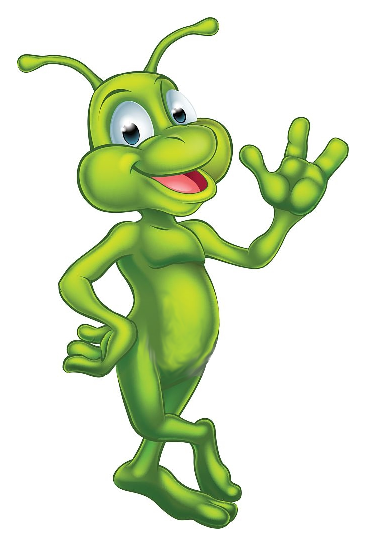
\includegraphics[width=2.8cm]{Nombres_et_calculs/Images/N1_ex_triomini}
   \end{minipage} \\
   Pour continuer à dénombrer, ils sont obligés de faire des regroupements par 3. \\
   Par exemple, voilà comment ils dénombrent cette quantité : \\
   \begin{pspicture}(0,0)(17,4.25)
      \psset{unit=0.7}
      \def\tri{\pspolygon(0,0)(2,0)(1,1.73)\rput(0.7,0.45){\ding{46}}\rput(1.3,0.45){\ding{46}}\rput(1,1){\ding{46}}}
      \multido{\n=1+1}{5}{\multido{\i=1+1}{5}{\rput(\n,\i){\ding{46}}}}
       \rput(7,3){$\Longrightarrow$}
       \rput(7.5,2){\tri} \rput(9.5,2){\tri} \rput(8.5,3.73){\tri} 
      \rput(12,2){\tri} \rput(14,2){\tri} \rput(13,3.73){\tri}
      \psbrace[ref=C,nodesepB=2mm](7.5,1.5)(16,1.5){\ding{108}}
      \rput(17,2){\tri} \rput(19.5,2){\tri}
      \psbrace[ref=C,nodesepB=2mm](17,1.5)(21.5,1.5){\ding{108}}
      \rput(23,2.5){\ding{46}}
      \psbrace[ref=C,nodesepB=2mm,rot=90](22.25,1.5)(23.75,1.5){\ding{115}}
   \end{pspicture}
   De la même manière, on a les correspondances suivantes :
   \begin{center}
      {\hautab{1.5}
      \begin{tabular}{|p{4cm}|C{2}|C{2}|C{2}|}
        \hline
         Numération décimale & 21 & 39 & 133 \\
         \hline
         Numération trimontoise & \ding{108}\,\ding{115}\,\ding{72} & \ding{115}\,\ding{115}\,\ding{115}\,\ding{72} & \ding{115}\,\ding{115}\,\ding{108}\,\ding{108}\,\ding{115}  \\
         \hline
      \end{tabular}}
   \end{center}
   \begin{enumerate}
      \item Caractériser ce système de numération.
      \item À partir de quel nombre, exprimé en écriture décimale, les triominis utilisent-ils quatre symboles ?
      \item Écrire dans notre numération le nombre triomontois suivant : \ding{108}\,\ding{115}\,\ding{72}\,\ding{115}\,\ding{72}.
      \item Écrire le nombre  que nous écrivons 143 en numération triomontoise.
      \item Quel nombre écrit en numération trimontoise vient juste avant \ding{115}\,\ding{72}\,\ding{108}\,\ding{72} ?
   \end{enumerate}
\end{exercice}

\begin{corrige}
\ \\ [-5mm]
   \begin{enumerate}
      \item Il s'agit d'un système {\blue positionnel de base 3}.
      \item Le premier nombre ayant quatre symboles est \ding{115}\,\ding{72}\,\ding{72}\,\ding{72} qui correspond à $1\times3^3 ={\blue 27}$.
      \item \ding{108}\,\ding{115}\,\ding{72}\,\ding{115}\,\ding{72} correspond au nombre $2\times3^4+1\times3^3+0\times3^2+1\times3^1+0\times3^0 ={\blue 192}$.
      \item On commence par écrire 143 en base 3, par exemple grâce aux divisions euclidiennes successives : \\
         $\opidiv[remainderstyle.2=\blue]{143}{3} \qquad \opidiv[remainderstyle.2=\blue]{47}{3} \qquad \opidiv[remainderstyle=\blue]{15}{3} \qquad \opidiv[remainderstyle=\blue]{5}{3} \qquad \opidiv[remainderstyle=\blue]{1}{3}$ \\ [1mm]
      On a donc $143 =\overline{12022}^3$ ce qui correspond à {\blue \ding{115}\,\ding{108}\,\ding{72}\,\ding{108}\,\ding{108}} en numération trimontoise.
      \item On peut effectuer la soustraction suivante : \begin{tabular}[t]{lllll}
         & & & \footnotesize\ding{115} & \footnotesize\ding{115}\ding{115}\ding{115} \\
         & \ding{115} & \ding{72} & \cancel{\ding{108}} & \ding{72} \\ [1mm]
         $-$ & & & & \ding{115} \\ [1mm]
         \cline{2-5}
         & \ding{115} & \ding{72} & \ding{115} & \ding{108} \\
      \end{tabular} \\ [1mm]
      Donc, le nombre qui vient juste avant \ding{115}\,\ding{72}\,\ding{108}\,\ding{72} est {\blue \ding{115}\,\ding{72}\,\ding{115}\,\ding{108}}
   \end{enumerate}
\end{corrige}


\bigskip


\begin{exercice}[CRPE 2005 Lille] %%% 4
   Dans la tribu des Cincofiles, on a une manière particulière de compter. Lors d'un voyage dans cette tribu, un chercheur a ramené un certain nombre d'observations qu'il a retranscrites dans un carnet. \\
   Voici ce qu'il a noté sur la manière de compter des Cincofiles :
   \begin{itemize}
      \item c'est une numération de position ;
      \item il n'y a que cinq symboles pour noter les nombres : \\
      \ding{108} pour notre 0, \quad \ding{121} pour notre 1, \quad \ding{54} pour notre 2, \quad \ding{116} pour notre 3, \quad \ding{110} pour notre 4 ; \\ [-5mm]
      \item une observation : \\
         {\psset{dotstyle=diamond,dotscale=2,unit=0.7}
         \begin{pspicture}(0,0)(16,6)       
            \psRandom[randomPoints=39](0,0)(6,5){}
            \rput(7,3){\Large$\Longrightarrow$}
            \psframe[linestyle=dashed](8,0)(18.5,6)
            \psframe(8.5,0.5)(13.5,5.5)
            \multido{\n=9+1}{5}{\multido{\i=1+1}{5}{\psdot(\n,\i)}}
            \psline[linestyle=dashed](14,0)(14,6)
            \psframe(14.5,0.5)(15.5,5.5)
            \multido{\i=1+1}{5}{\psdot(13,\i)}
            \psframe(16,0.5)(17,5.5)
            \multido{\i=1+1}{5}{\psdot(16.5,\i)}
            \psline[linestyle=dashed](17.5,0)(17.5,6)
            \multido{\i=1+1}{4}{\psdot(18,\i)}
            \rput(19.5,3){\Large$\Longrightarrow$}
            \rput(21,3){\ding{121} \ding{54} \ding{110}}
         \end{pspicture}} \\
      \item des exemples de transcriptions : \quad {\hautab{1.5}
      \begin{ttableau}{0.5\linewidth}{4}
         \hline
         \ding{121} \ding{116} & \ding{110} \ding{54} & \ding{54} \ding{108} \ding{110} & \ding{121} \ding{121} \ding{116} \ding{110} \\
         \hline
         8 & 22 & 54 & 169 \\
         \hline
      \end{ttableau}}
   \end{itemize} 
   \begin{enumerate}
      \item En expliquant votre démarche :
      \begin{enumerate}
         \item Transcrire dans notre système de numération le nombre noté par les Cincofiles \og \ding{110} \ding{110} \ding{110} \fg.
         \item Transcrire dans le système Cincofile le nombre que nous notons \og 273 \fg.
      \end{enumerate}
      \item Sans passer par une transcription dans notre système de numération décimale, écrire :
      \begin{enumerate}
         \item Le nombre qui précède le nombre \og \ding{116} \ding{110} \ding{108} \fg{} dans le système Cincofile ?
         \item Le nombre qui suit le nombre \og \ding{54} \ding{110} \ding{110} \fg{} dans le système Cincofile ?
      \end{enumerate}
       Ces deux derniers nombres seront donnés en écriture Cincofile.
   \end{enumerate}
\end{exercice}

\begin{corrige}
\ \\ [-5mm]
   \begin{enumerate}
      \item 
      \begin{enumerate}
         \item Le système Cincofile est un système de numération positionnel de base 5. \\
         Dans notre système positionnel de base 10, \, \ding{110} \ding{110} \ding{110} est représenté par le nombre $4\times5^2+4\times5^1+4\times5^0 =4\times25+4\times5+4 ={\blue 124}.$
      \end{enumerate}
   \textcolor{G1}{\bf b)} On effectue les divisions euclidiennes successives par 5 : \\
      $\opidiv[remainderstyle.2=\textcolor{blue}]{273}{5}$ \quad $\opidiv[remainderstyle.2=\textcolor{blue}]{54}{5}$ \quad $\opidiv[remainderstyle=\textcolor{blue}]{10}{5}$ \quad $\opidiv[remainderstyle=\textcolor{blue}]{2}{5}$. \\ [1mm]
      Donc, 273 s'écrit $\overline{2043}^5$ en base 5, ce qui est codé par \, {\blue\ding{54} \ding{108} \ding{110} \ding{116}} \\
      \setcounter{enumi}{1}
      \item
      \begin{enumerate}
          \item On doit enlever une unité au nombre \ding{116} \ding{110} \ding{108} \\
            Or, le chiffre du premier rang (rang des unités) est nul, on va donc \og prendre \fg{} une unité au rang 2 (que l'on pourrait appeler rang des quinaires) que l'on va ajouter au rang 1, auquel on peut cette fois-ci supprimer une unité, il restera donc \ding{110} alors qu'au deuxième rang, \ding{110} sera devenu \ding{116} \\
Le nombre recherché est donc {\blue \ding{116} \ding{116} \ding{110}}
            \item On ajoute une unité au premier rang \ding{110} qui nous donne \og 5 \fg, donc une unité de rang 1 et une unité des quinaires (la retenue) en plus. \\
            Le chiffre de ce rang devient alors \ding{108} avec une unité supplémentaire au rang 3 : \ding{54} devient \ding{116} \\
            Le nombre suivant \og \ding{54} \ding{110} \ding{110} \fg{} est donc {\blue \ding{116} \ding{108} \ding{108}}
      \end{enumerate}
   \end{enumerate}
\end{corrige}


\bigskip


\begin{exercice}[Des nombres mystérieux] %%% 5
   Tous les nombres considérés dans cet exercice sont écrits dans la numération décimale. \\
   Déterminer les deux nombres mystère vérifiant les propriétés décrites.
\begin{enumerate}
   \item Premier nombre mystère :
      \begin{itemize}
         \item son chiffre des unités est égal à 5 ;
         \item il a 431 centaines ;
         \item son chiffre des dizaines est égal à 2.
      \end{itemize}
   \item Deuxième nombre mystère :
      \begin{itemize}
         \item il est compris entre 15 000 et 16 000 ;
         \item tous ses chiffres sont différents ;
         \item son chiffre des centaines est un multiple de 3 ;
         \item son chiffre des unités est un nombre pair supérieur à 5 ;
         \item son chiffre des dizaines est le successeur du chiffre des centaines et est la moitié du chiffre des unités.
      \end{itemize}
   \end{enumerate}
\end{exercice}

\begin{corrige}
\ \\ [-5mm]
   \begin{enumerate}
      \item Le premier nombre mystère est {\blue 43\,125}.
      \item Le second nombre mystère est {\blue 15\,348}.
   \end{enumerate}
\end{corrige}


\bigskip


\begin{exercice}[CRPE 2001 Aix] %%% 6
\ \\ [-10mm]
   \begin{enumerate}
      \item Voici deux propositions concernant des nombres entiers donnés en écriture décimale. Dire pour chacune d'elles si elle est vraie ou fausse et justifier. \\
          A : si l'écriture d'un nombre se termine par 2, alors l'écriture du carré de ce nombre se termine par 4. \\
         B : si l'écriture d'un nombre se termine par 4, alors l'écriture du carré de ce nombre se termine par 16
      \item L'écriture d'un nombre entier $n$ est de la forme $\overline{a5}$ où $a$ est le chiffre des dizaines, différent de 0. \\
         Démontrer que $n^2$ s'écrit avec 4 chiffres au plus. \\
         Démontrer que l'écriture de $n^2$ se termine par 25 et que le nombre de centaines de $n^2$ est égal à $a(a+1)$.
   \end{enumerate}
\end{exercice}

\begin{corrige}
\ \\ [-5mm]
   \begin{enumerate}
      \item 
      {\blue La proposition A est vraie} \\
         Soit $n$ un nombre se terminant par 2, il s'écrit $n=10k+2$ où $k$ est le nombre de dizaines de $n$. \\
         On a alors : $n^2 =(10k+2)^2$ \\
         \hspace*{2.1cm} $=100k^2+40k+4$ \\
         \hspace*{2.1cm} $=10(10k^2+4k)+4$. \\
         On reconnait l'écriture d'un nombre décimal où le chiffre des unités est 4. \\      
      {\blue La proposition B est fausse.} \\
       Il suffit de donner un contre-exemple : $14^2=196$ ne se termine pas par 16. \\
      \item $n =\overline{a5} =10a+5$. Donc, $n^2=(10a+5)^2$ \\
      \hspace*{4.35cm} $=100a^2+100a+25$ \\
      \hspace*{4.35cm} $ =100(a^2+a)+25$. \\
      On en déduit les choses suivantes :
      \begin{itemize}
         \item le maximum de $n^2$ est $100(9^2+9)+25 =9025$ qui s'écrit avec {\blue 4 chiffres} ; \\
         \item $n^2$ est composé de $a^2+a =${\blue $a(a+1)$} centaines additionné de 25, donc {\blue il se termine par 25}. \\
      \end{itemize}
   \end{enumerate}
\end{corrige}


\bigskip


\begin{exercice}[CRPE 2018 G2] %%% 7
   Pour calculer de tête le carré d'un nombre entier se terminant par 5 :
   \begin{itemize}
      \item on prend le nombre de dizaines et on le multiplie par l’entier qui suit ce nombre de dizaines, cela donne le nombre de centaines du résultat ;
      \item on écrit ensuite 25 à droite du nombre de centaines pour obtenir le résultat.
   \end{itemize}
   Par exemple, 105 est composé de 10 dizaines et 5 unités, son carré.   s'obtient :
   \begin{itemize}
      \item étape 1 : en calculant $10\times11 =110$, ce qui donne le nombre de centaines du
résultat ;
      \item étape 2 : on écrit ensuite 25 à droite de 110 pour obtenir le résultat.
   \end{itemize}
   On a donc $105^2 = 11\,025$.
   \begin{enumerate}
      \item Montrer comment calculer mentalement $45^2$.
      \item Soit $n$ un nombre entier se terminant par 5, $n$ peut s’écrire : $10d+5$ avec $d$ le nombre de dizaines. \\
         Établir la relation : $n^2 =100d(d+1)+25$.
      \item Grâce au résultat de la question 2),  justifier la technique de calcul mental présentée dans l’énoncé.
      \item Comment, par extension de la technique de calcul mental présentée, calculer mentalement le carré de 3,5 ?
   \end{enumerate}
\end{exercice}

\begin{corrige}
\ \\ [-5mm]
   \begin{enumerate}
      \item 45 est composé de 4 dizaines et de 5 unités.
      \begin{itemize}
         \item Étape 1 : on calcule $4\times5 =20$ ce qui correspond au nombre de centaines.
         \item Étape 2 : on écrit 25 à droite de 20. 
      \end{itemize}
      On a donc {\blue $45^2 =2\,025$.}
      \item $n^2 =(10d+5)^2$ \\
        \hspace*{0.8cm} $=(10d)^2+2\times10d\times5+5^2$ \\
         \hspace*{0.8cm} $=100d^2+100d+25$ \\
         \hspace*{0.4cm} {\blue $n^2 =100d(d+1)+25.$}
   \end{enumerate}
   
\Coupe

   \begin{enumerate}
   \setcounter{enumi}{2}
      \item Le terme \og $d(d+1)$ \fg{} correspond à la multiplication du nombre de dizaines $d$ par l'entier qui le suit $(d+1)$. Le résultat obtenu est multiplié par 100 ce qui signifie que $d(d+1)$ est le nombre de centaines (étape 1) ; \\
         à ce nombre, on ajoute 25 qui est un nombre inférieur à 100 c'est la raison pour laquelle il suffit d'écrire 25 à droite du nombre de centaines pour obtenir le résultat (étape 2).
      \item Un nombre décimal $n'$ de partie décimale 5 peut s'écrire sous la forme de la fraction décimale $n' =\dfrac{n}{10}$ où $n$ est un nombre entier qui se termine par 5. \\
         On a alors $n' =\dfrac{n^2}{100} =\dfrac{100d(d+1)+25}{100} =d(d+1)+0,25$. \\ [1mm]
         Par analogie avec ce qui a été vu pour les entiers, il suffit donc de multiplier la partie entière par son successeur pour obtenir la partie entière et de prendre 25 comme partie décimale. \\
         Si on applique ce procédé à 3,5, on effectue le produit de 3 par 4 qui donne 12 (partie entière) et 25 est la partie décimale donc : {\blue $3,5^2 =12,25$.}
   \end{enumerate}
\end{corrige}


\bigskip


\begin{exercice}[CRPE 2022 Sujet 0] %%% 8
   Soit $M$ un nombre entier naturel inférieur à 100. On note $u$ le chiffre des unités du nombre $M$ et $d$ son chiffre des dizaines. \\
   Soit $N$ un nombre entier naturel inférieur à 100, ayant le même chiffre $d$ des dizaines que $M$ et tel que son chiffre $v$ des unités vérifie $u+v =10$. \\
   Par exemple, pour $M =34$, alors $N =36$ vérifie ces conditions. \\
   Pour $M$ et $N$ vérifiant les conditions ci-dessus, on propose d’utiliser l’algorithme ci-dessous pour calculer le produit $M\times N$.
  \begin{center}
     \fbox{
     \begin{minipage}{13cm}
        {\bf Algorithme de calcul} \\
           -- On calcule le produit de $d$ et de l’entier suivant $d+1$. \\
           -- On calcule le produit de $u$ et de $v$. \\
           -- On ajoute au produit de $u$ et de $v$, 100 fois le produit de $d$ et de l’entier suivant $d+1$.
     \end{minipage}
     }
  \end{center}
  \begin{enumerate}
     \item Vérifier en détaillant les calculs que cet algorithme fonctionne pour $34\times36$.
      \item Démontrer que cet algorithme de calcul donne effectivement le résultat escompté pour tous les couples de nombres $M$ et $N$ vérifiant les conditions mentionnées en début d’exercice. \\
      On pourra utiliser les égalités $M =10d+u$ et $N =10d+v$.
      \item Montrer comment on peut utiliser cet algorithme de calcul, en détaillant les calculs, pour calculer mentalement $4,2\times4,8$.
  \end{enumerate}
\end{exercice}

\begin{corrige}
\ \\ [-5mm]
   \begin{enumerate}
      \item On a $M =34$ et $N =36$, donc $d =3 ; u =4$ et $v =6$. \\
         $\bullet \; d\times(d+1) =3\times4 =12$. \\
         $\bullet \; u\times v =4\times6 =24$. \\
         $\bullet \; 100\times d(d+1)+uv =100\times12+24 =1\,224$. \\
         D'un autre côté, $34\times36 =1\,224$. Donc, {\blue l'algorithme fonctionne pour $34\times36$}.
      \item $M\times N =(10d+u)\times(10d+v)$ \\
         \hspace*{1.47cm} $=10d\times10d+10d\times v+u\times10d+u\times v$ \\
         \hspace*{1.47cm} $=100d^2+10d(v+u)+uv$ \\
         \hspace*{1.47cm} $=100d^2+10d\times10+uv$ \\
         \hspace*{1.47cm} $=100d^2+100d+uv$ \\
         \hspace*{0.36cm} {\blue $M\times N =100d(d+1)+uv.$} \smallskip
      \item $4,2\times4,8 =\dfrac{42}{10}\times\dfrac{48}{10} =\dfrac{42\times48}{100}$. \\ [1mm]
         On applique l'algorithme à $42\times48$ avec $d =4 ; u =2$ et $v =8$ : \\
         $\bullet \; d\times(d+1) =4\times5 =20$. \\
         $\bullet \; u\times v =2\times8 =16$. \\
         $\bullet \; 100\times d(d+1)+uv =100\times20+16 =2\,016$. \\ [1mm]
         Donc : {\blue $4,2\times4,8 =\dfrac{2\,016}{100} =20,16$}.
      \end{enumerate}
\end{corrige}
 
 
\bigskip
 
 
\begin{exercice}[CRPE 2003 Guadeloupe] %%% 9
   On cherche à déterminer un nombre à trois chiffres dont la somme est 16. \\
   Si l'on intervertit le chiffre des centaines et celui des dizaines, le nombre augmente de 450 et si l'on intervertit le chiffre des centaines et celui des unités il augmente de 198. \\
   Déterminer ce nombre.
\end{exercice}

\begin{corrige}
   Soit N $=\overline{cdu}$ le nombre recherché.
   \begin{itemize}
      \item La somme de ses chiffres est 16 donc, $c+d+u =16$. \quad{\it (1)} \\
      \item Si l'on intervertit le chiffre des centaines et celui des dizaines, le nombre augmente de 450 :
      \begin{align*}
         \overline{dcu} =\overline{cdu}+450 & \iff 100d+10c+\cancel{u} =100c+10d+\cancel{u}+450 \\ 
         & \iff 100d-10d-100c+10c =450 \\
         & \iff 90d-90c=450 \\
         & \iff 9d-9c =45 \\
         & \iff d-c =5 \\
         & \iff d=c+5 \quad {\it (2)}
      \end{align*}
   \end{itemize}
   
\Coupe

   \begin{itemize}
      \item Si l'on intervertit le chiffre des centaines et celui des unités, il augmente de 198 :
      \begin{align*}
         \overline{udc} =\overline{cdu}+198 & \iff 100u+\cancel{10d}+c =100c+\cancel{10d}+u+198 \\
         & \iff 100u-u-100c+c =198 \\
         & \iff 99u-99c =198 \\
         & \iff u-c =2 \\
         & \iff u =c+2 \quad {\it (3)}
      \end{align*}
   \end{itemize}
   Dans {\it (1)}, on remplace $d$ et $u$ obtenus en {\it (2)} et {\it (3)} :
   \begin{align*}
   c+(c+5)+(c+2)=16 & \Longleftrightarrow c+c+5+c+2=16 \\
   & \Longleftrightarrow 3c=9 \\
   & \Longleftrightarrow c=3
   \end{align*}
   On a alors d'après {\it (2)} : $d=3+5=8$ et d'après {\it (3)} : $u=3+2=5$. \\
   Le nombre recherché est {\blue $N = 385$}. \\
\end{corrige}


\bigskip

  
\begin{exercice}[Quel charabia !] %%% 10
   Compléter le tableau suivant en considérant la numération maya comme une numération de base 20. \\ [2mm]
   {\hautab{2}
   \setlength{\tabcolsep}{1mm}
   \begin{cltableau}{1\linewidth}{7}
      \hline
      & 12 & & & & & \\
      \hline
      & & & & & & \\
      Égyptien & \Large\textpmhg{\Hten\Hone\Hone} & \Large\textpmhg{\Hten\Hten\Hten\Hten} & & & & \\
      & & & & & & \\ [1mm]
      \hline
      Romain & \large\cRm{12} & & \large\cRm{248} &  & & \\
      \hline
      & 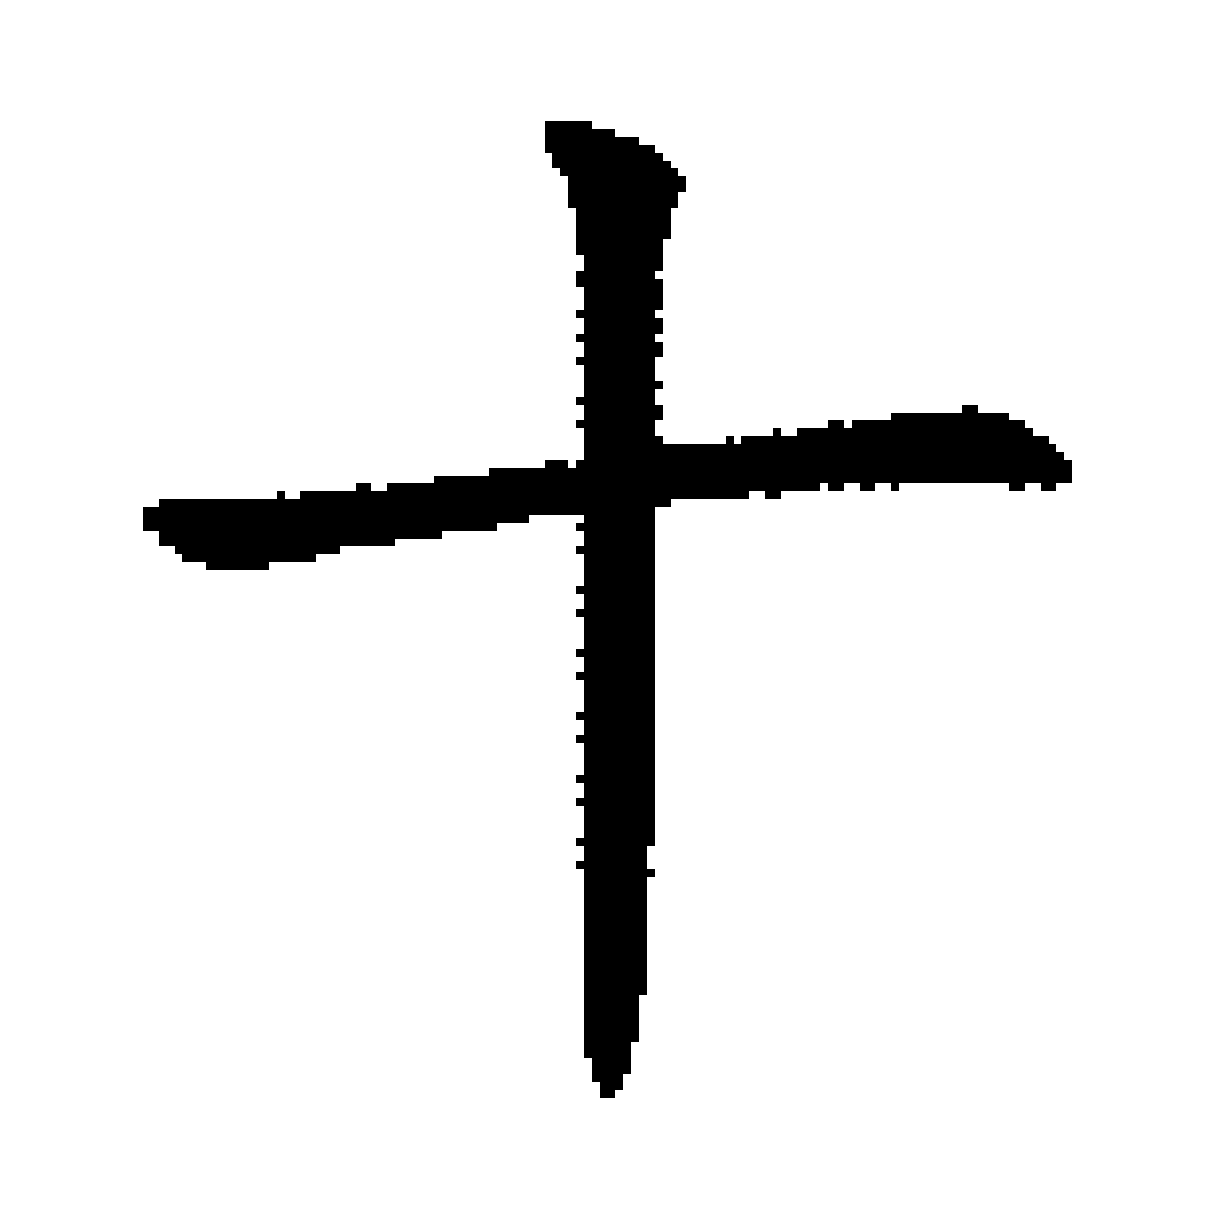
\includegraphics[width=5mm]{Nombres_et_calculs/Images/N1_chinois10.eps}  & &  & 
\includegraphics[width=5mm]{Nombres_et_calculs/Images/N1_chinois3} & & \\
      & 
\includegraphics[width=6mm]{Nombres_et_calculs/Images/N1_chinois2} & &  & 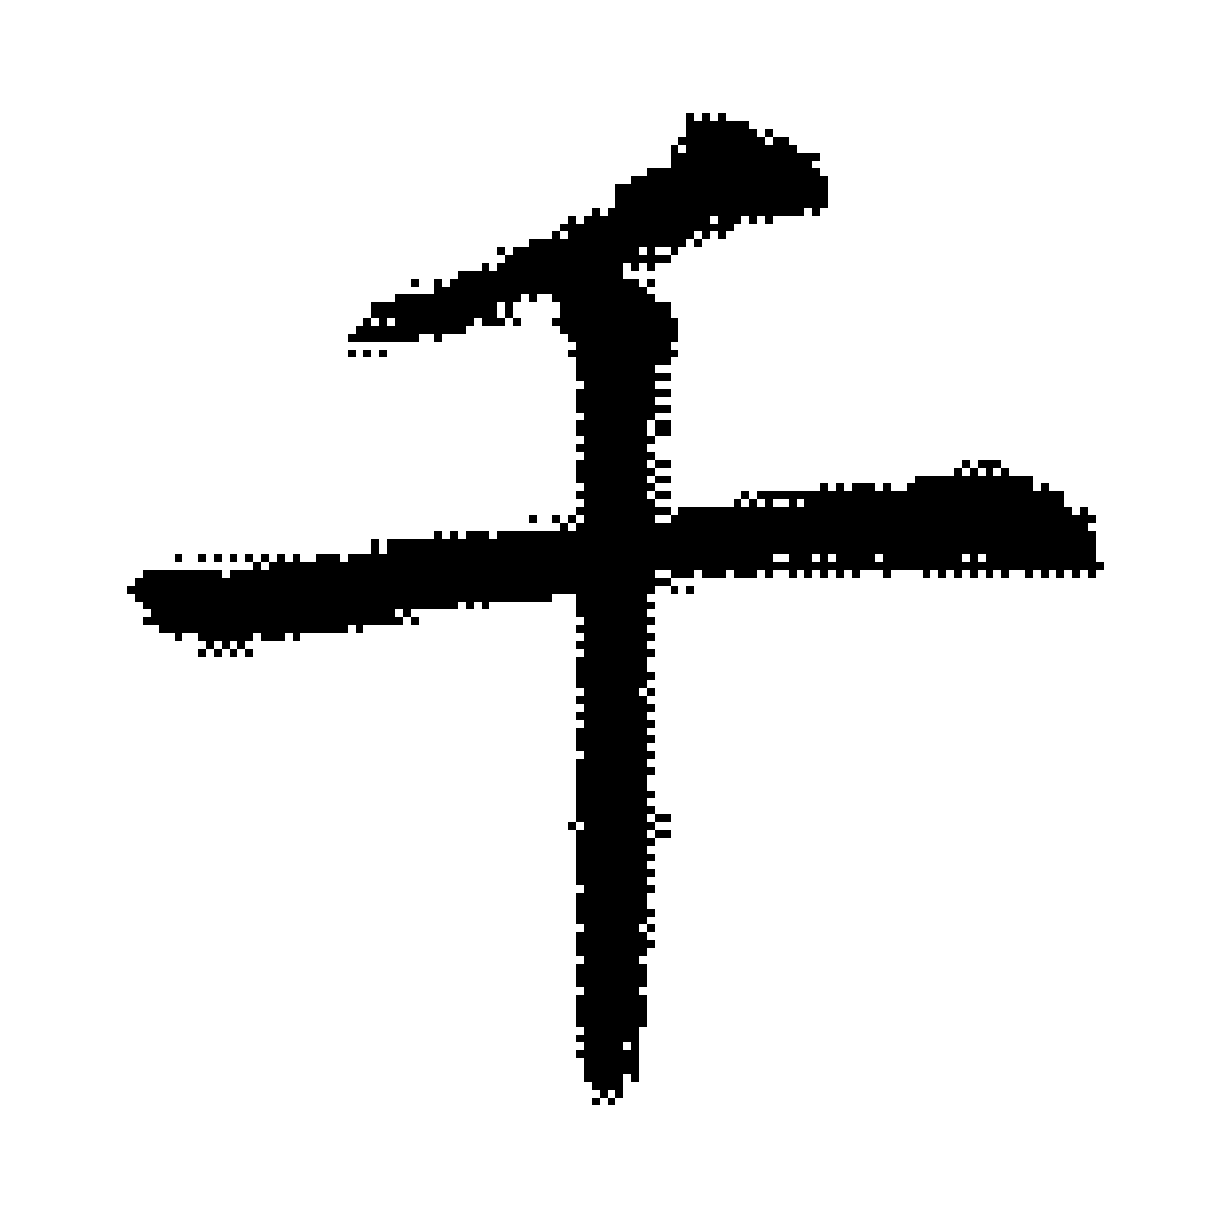
\includegraphics[width=5mm]{Nombres_et_calculs/Images/N1_chinois1000} & & \\
      \small\bf Chinois & & &  & 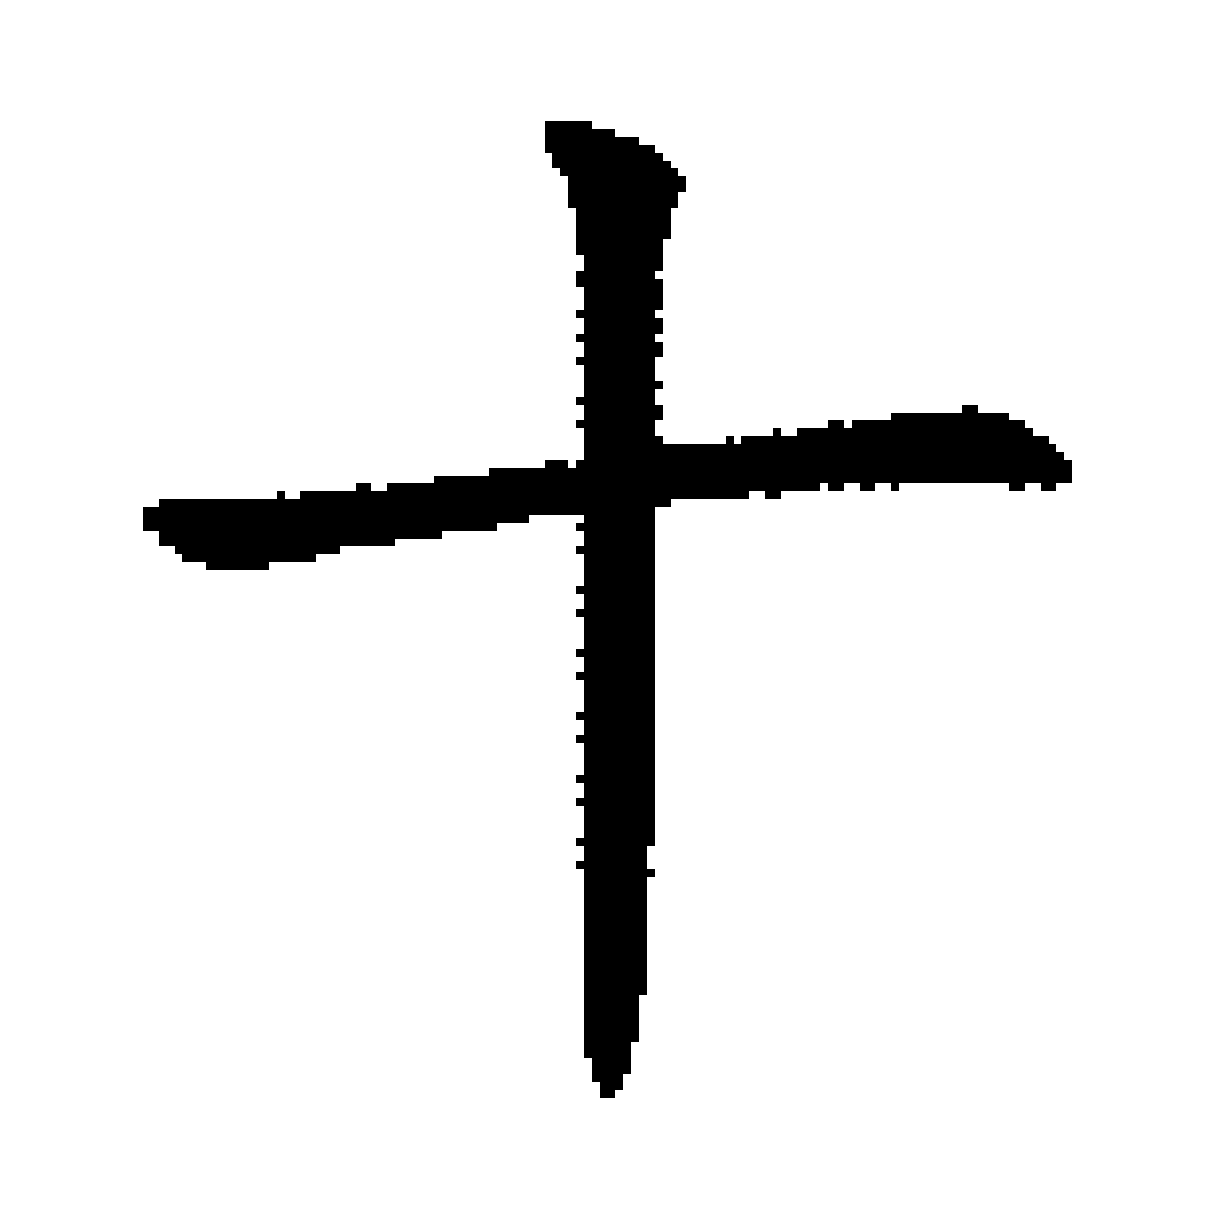
\includegraphics[width=5mm]{Nombres_et_calculs/Images/N1_chinois10} & & \\
      & & & & 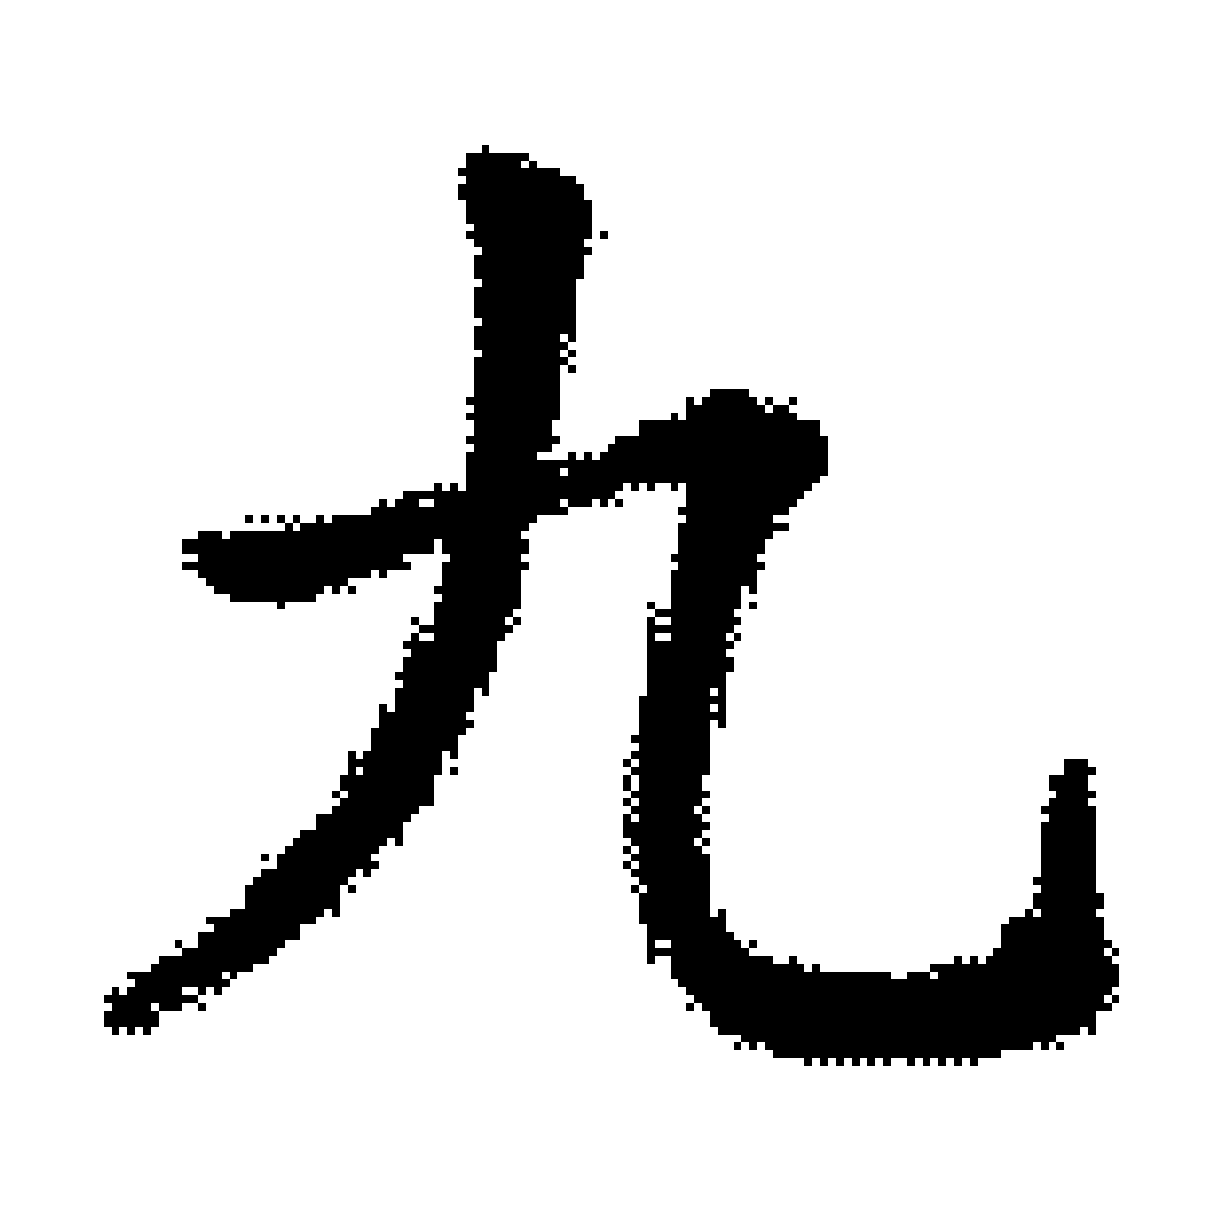
\includegraphics[width=5mm]{Nombres_et_calculs/Images/N1_chinois9} & & \\
      & & &  & & & \\ 
      \hline
      & & &  & & & \\ [-7mm]
      Maya & $\Large\maya{12}$ & & &  & $\Large\maya{1002}$ & \\ [18mm]
      \hline
      Binaire & & & & & & 1111101011 \\
      \hline
   \end{cltableau}}
\end{exercice}

\begin{corrige}
\ \\ [-3mm]
   {\hautab{1.5}
   {\setlength{\tabcolsep}{1mm}
   \begin{cltableau}{1\linewidth}{7}
      \hline
      & 12 & 40 & 248 & 3 019 & 1 002 & 1 003 \\
      \hline
      & & & \large\textpmhg{\Hhundred\Hhundred} & \multirow{2}{*}{\large\textpmhg{\Hthousand\Hthousand\Hthousand}} & \multirow{3}{*}{\large\textpmhg{\Hthousand\Hone\Hone}} & \multirow{3}{*}{\large\textpmhg{\Hthousand\Hone\Hone\Hone}} \\
      Égyptien & \large\textpmhg{\Hten\Hone\Hone} & \large\textpmhg{\Hten\Hten\Hten\Hten} & \large\textpmhg{\Hten\Hten\Hten\Hten} & & & \\
      & & & \large\textpmhg{\Hone\Hone\Hone\Hone\Hone\Hone\Hone\Hone} & \large\textpmhg{\Hten\Hone\Hone\Hone\Hone\Hone\Hone\Hone\Hone\Hone} & & \\
      \hline
      Romain & \cRm{12} & \cRm{40} & \cRm{248} & \cRm{3019} & \cRm{1002} & \cRm{1003} \\
      \hline
      & 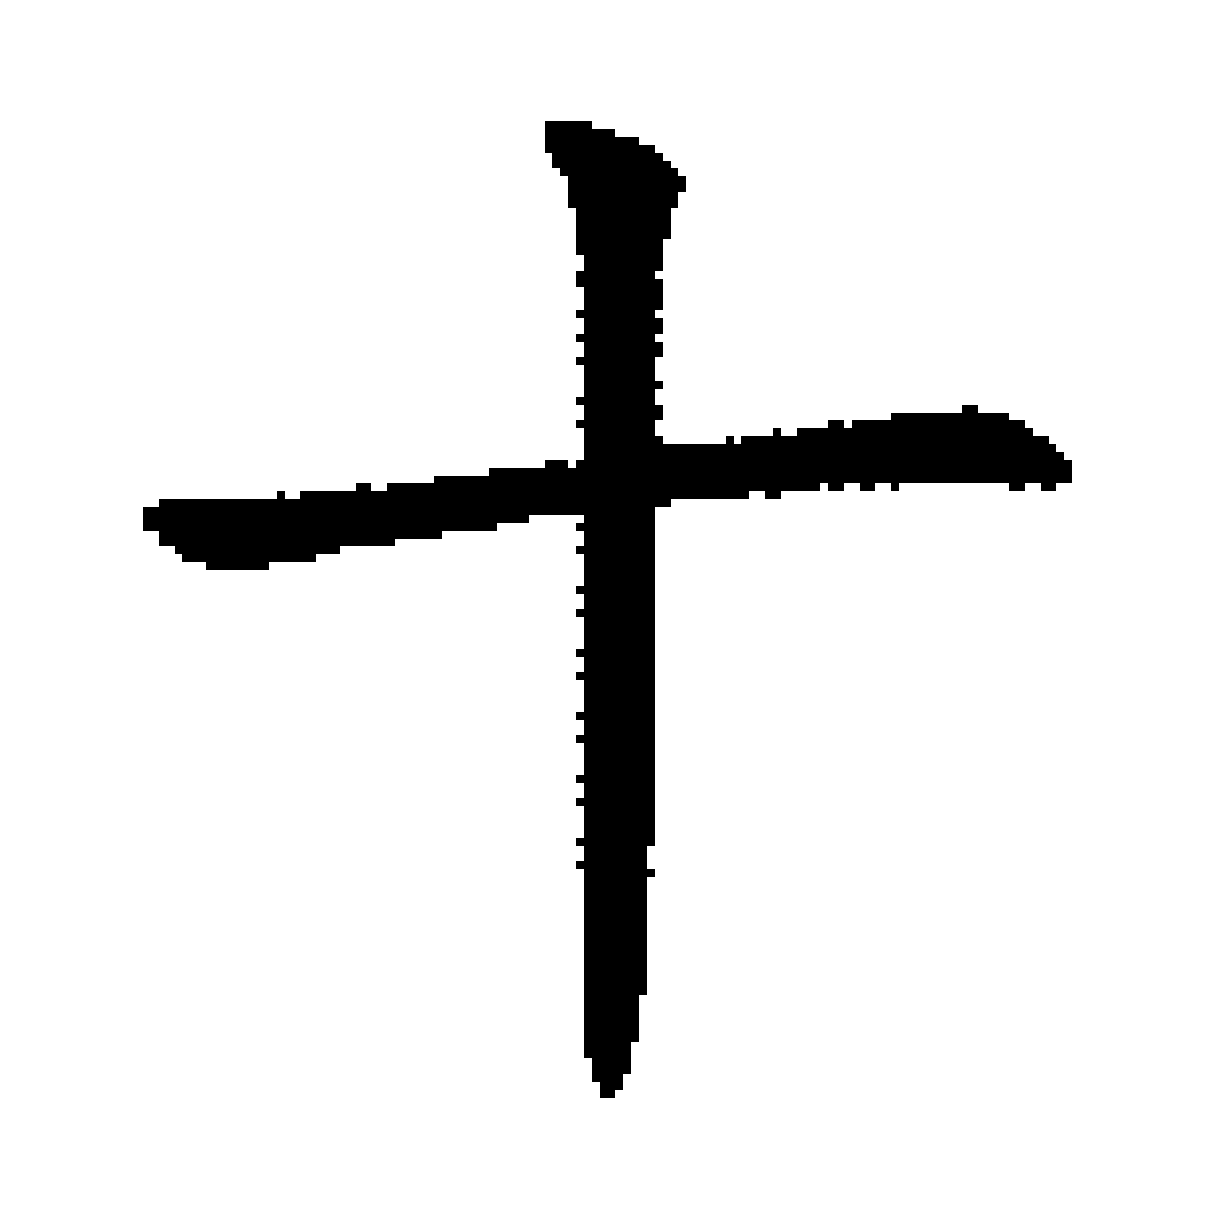
\includegraphics[width=5mm]{Nombres_et_calculs/Images/N1_chinois10} & 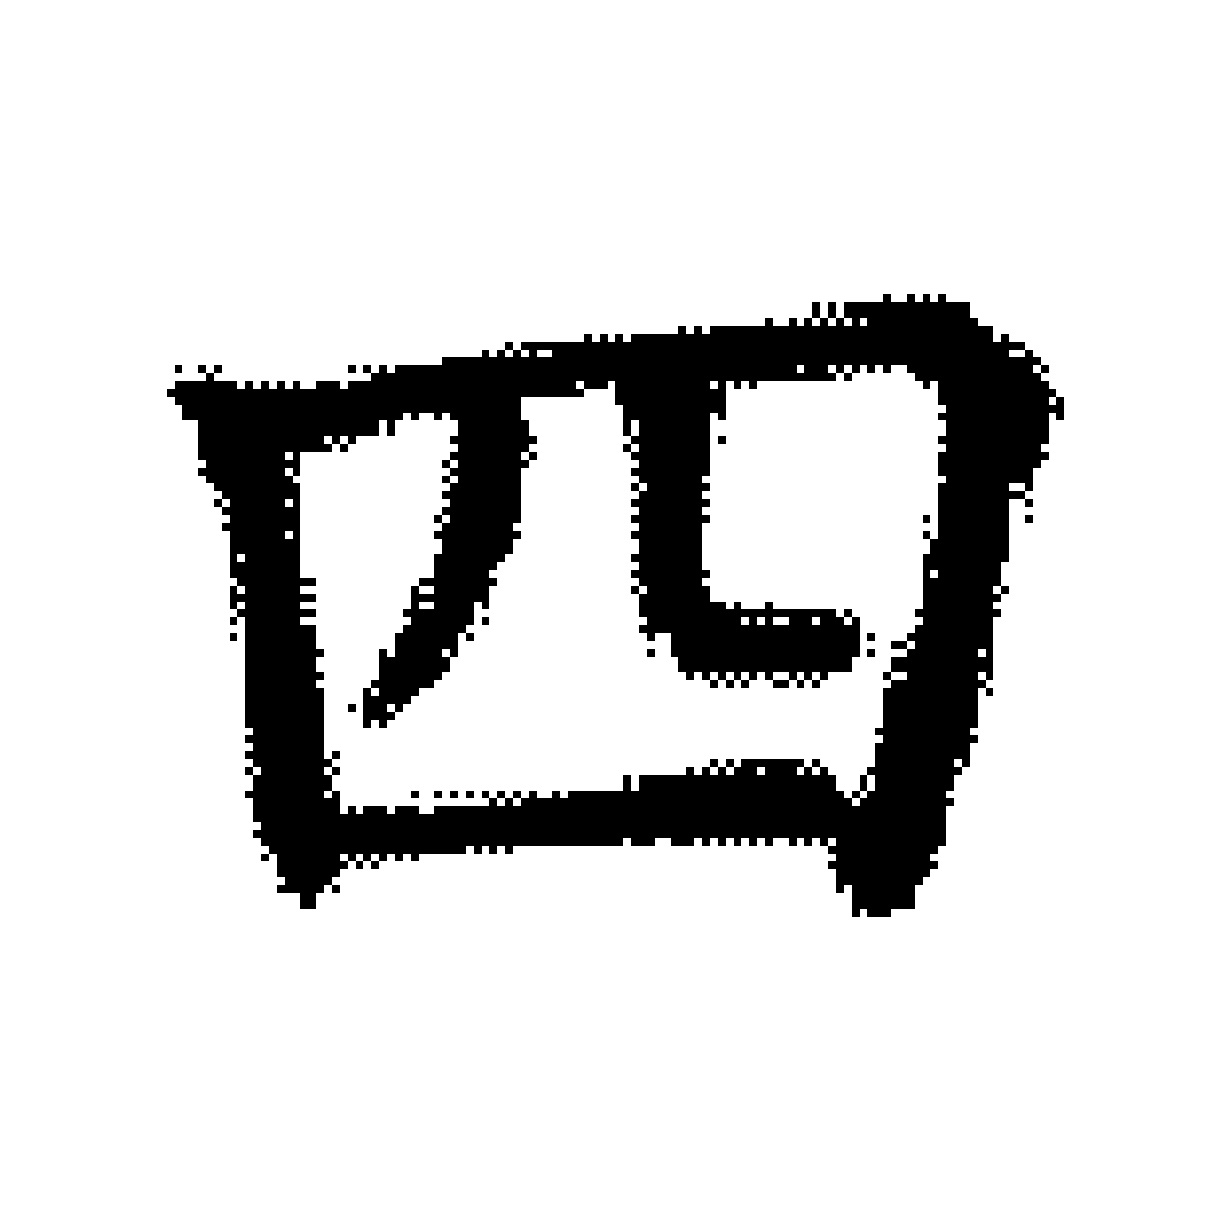
\includegraphics[width=5mm]{Nombres_et_calculs/Images/N1_chinois4} & 
\includegraphics[width=5mm]{Nombres_et_calculs/Images/N1_chinois2} & 
\includegraphics[width=5mm]{Nombres_et_calculs/Images/N1_chinois3} & 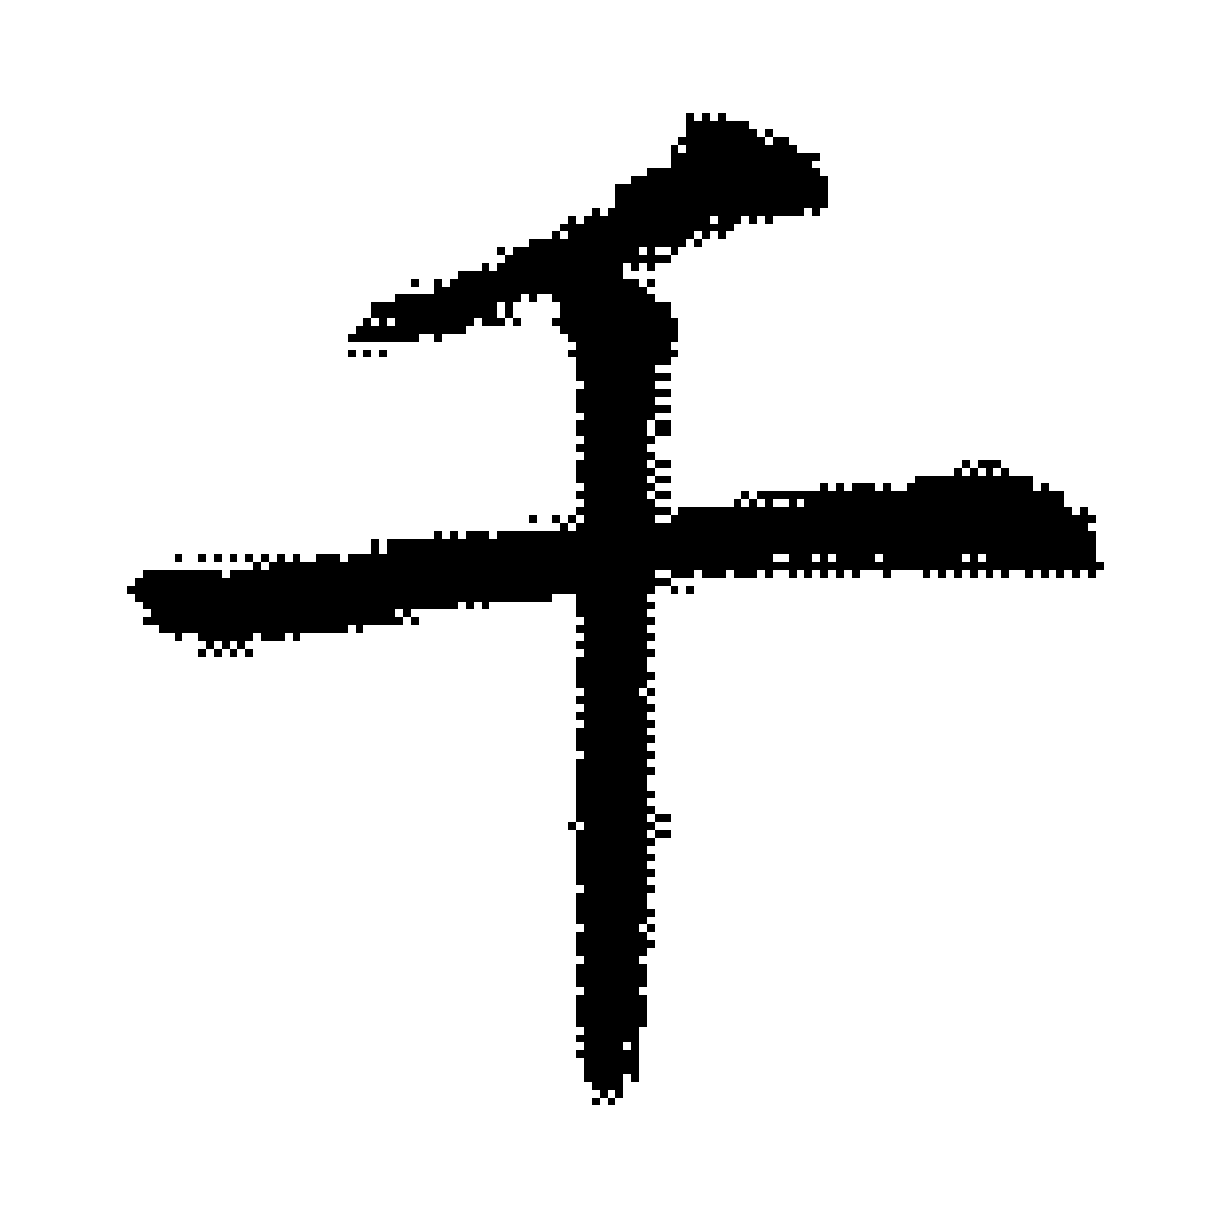
\includegraphics[width=5mm]{Nombres_et_calculs/Images/N1_chinois1000} & 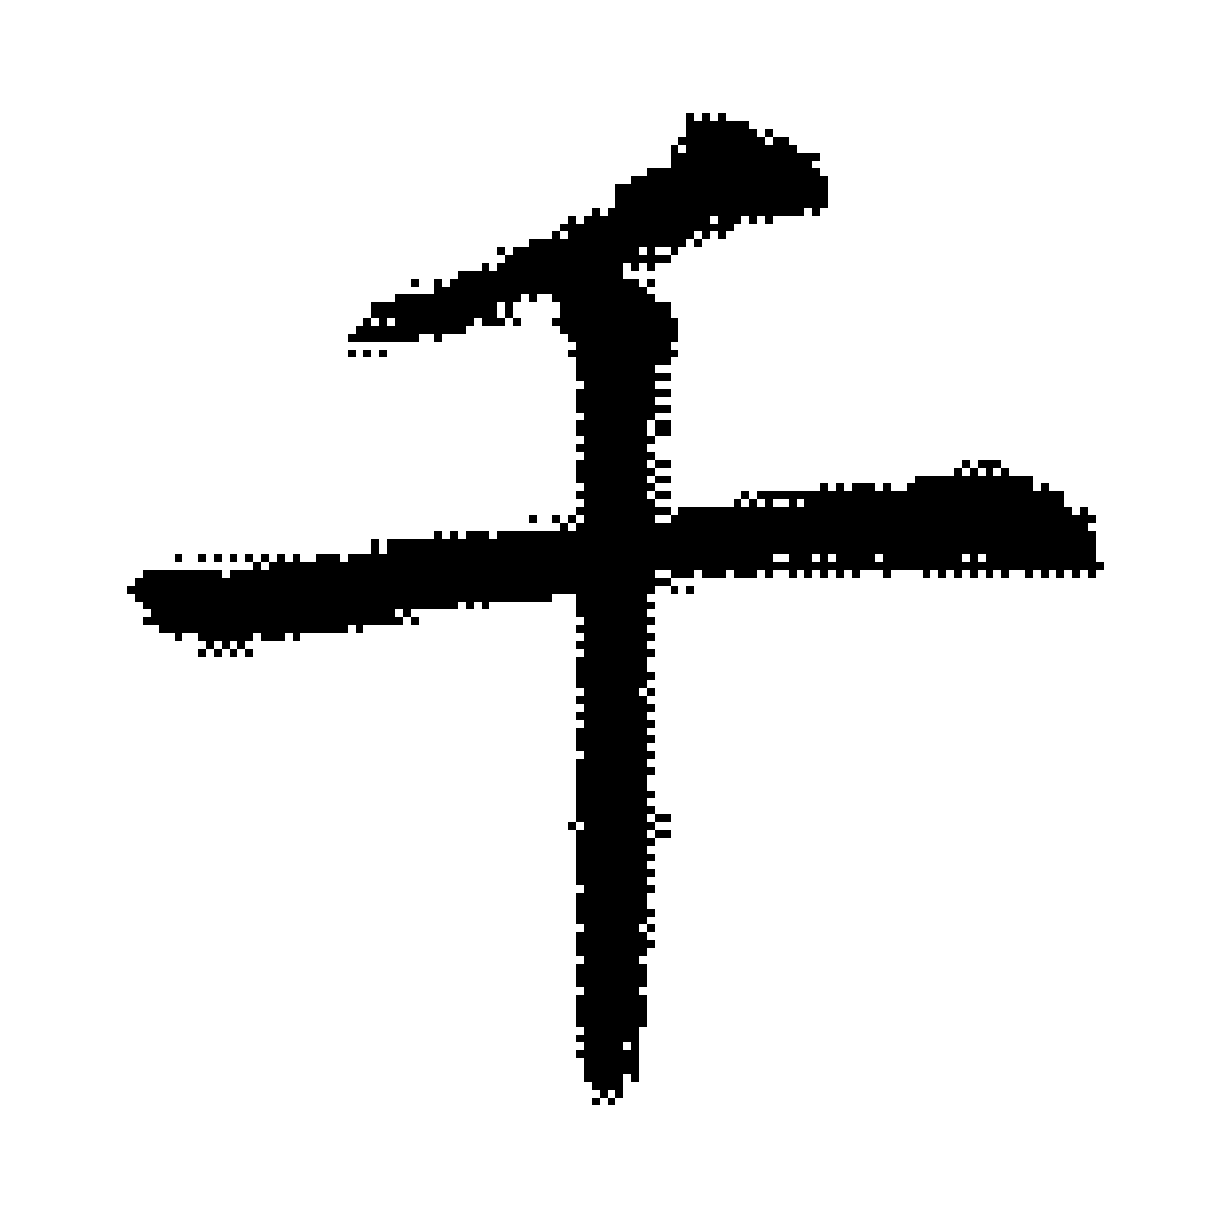
\includegraphics[width=5mm]{Nombres_et_calculs/Images/N1_chinois1000} \\
      & 
\includegraphics[width=5mm]{Nombres_et_calculs/Images/N1_chinois2} & 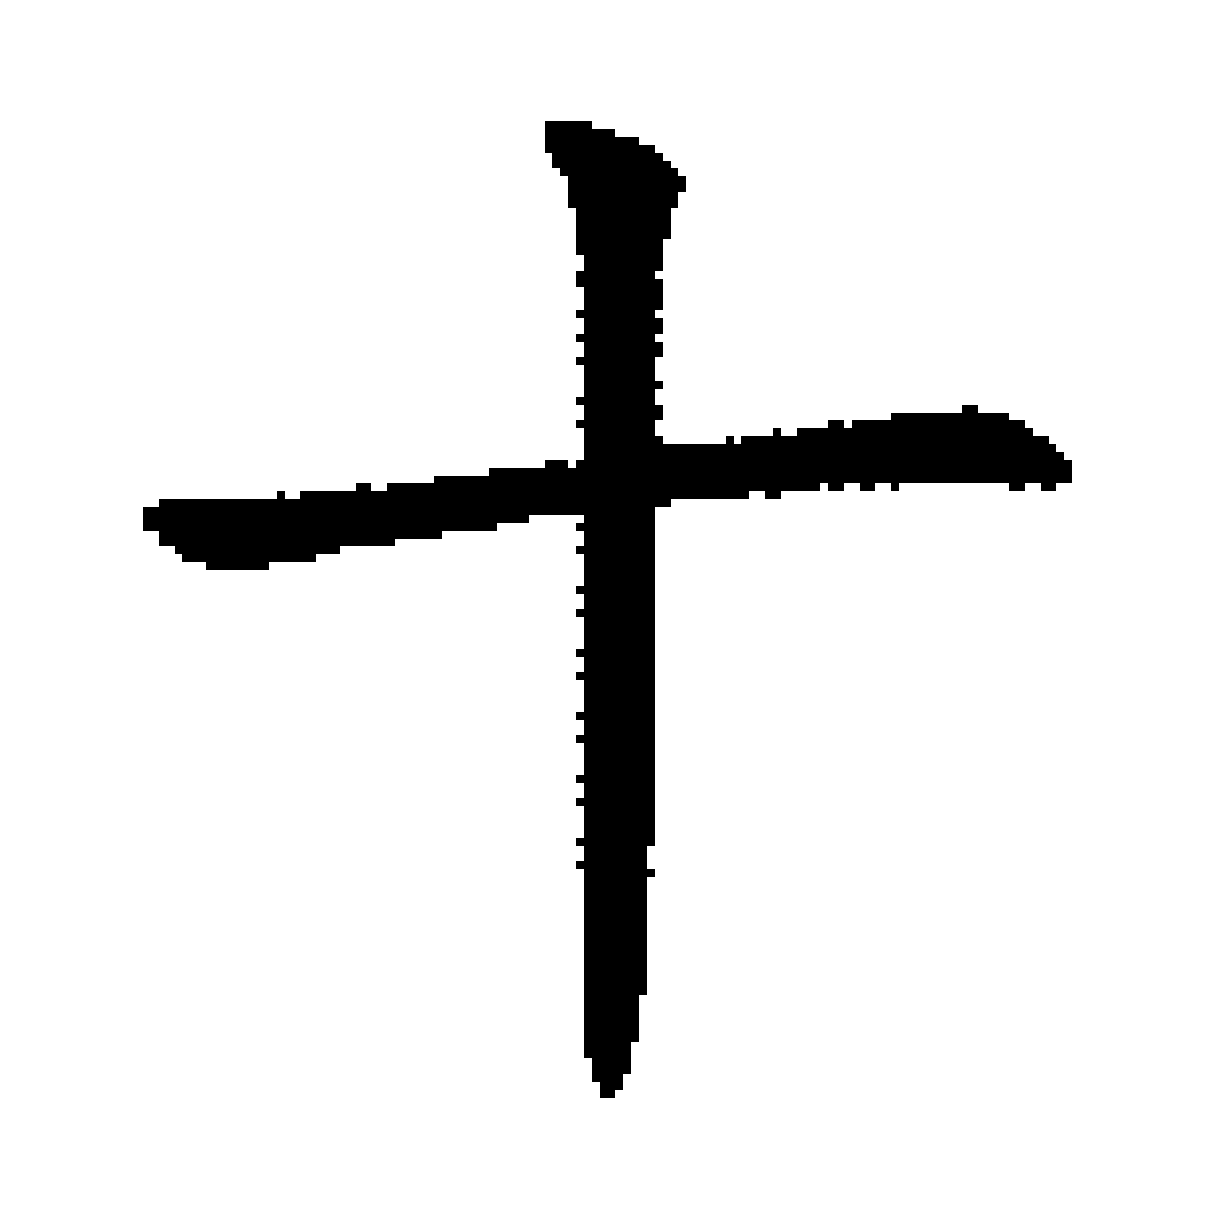
\includegraphics[width=5mm]{Nombres_et_calculs/Images/N1_chinois10} & 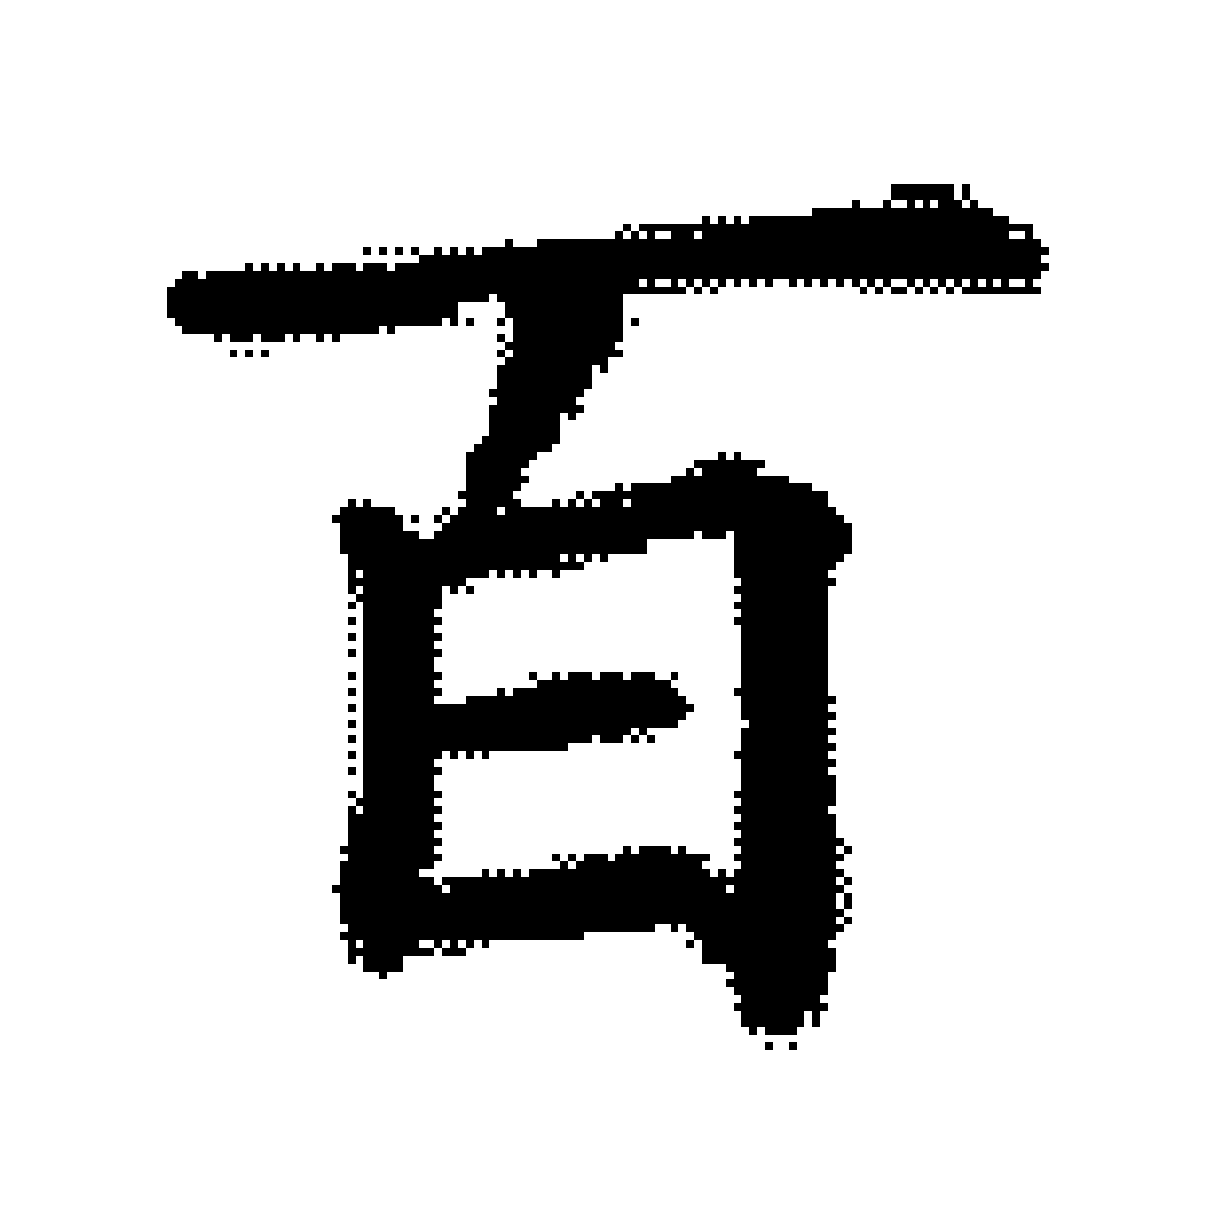
\includegraphics[width=5mm]{Nombres_et_calculs/Images/N1_chinois100} & 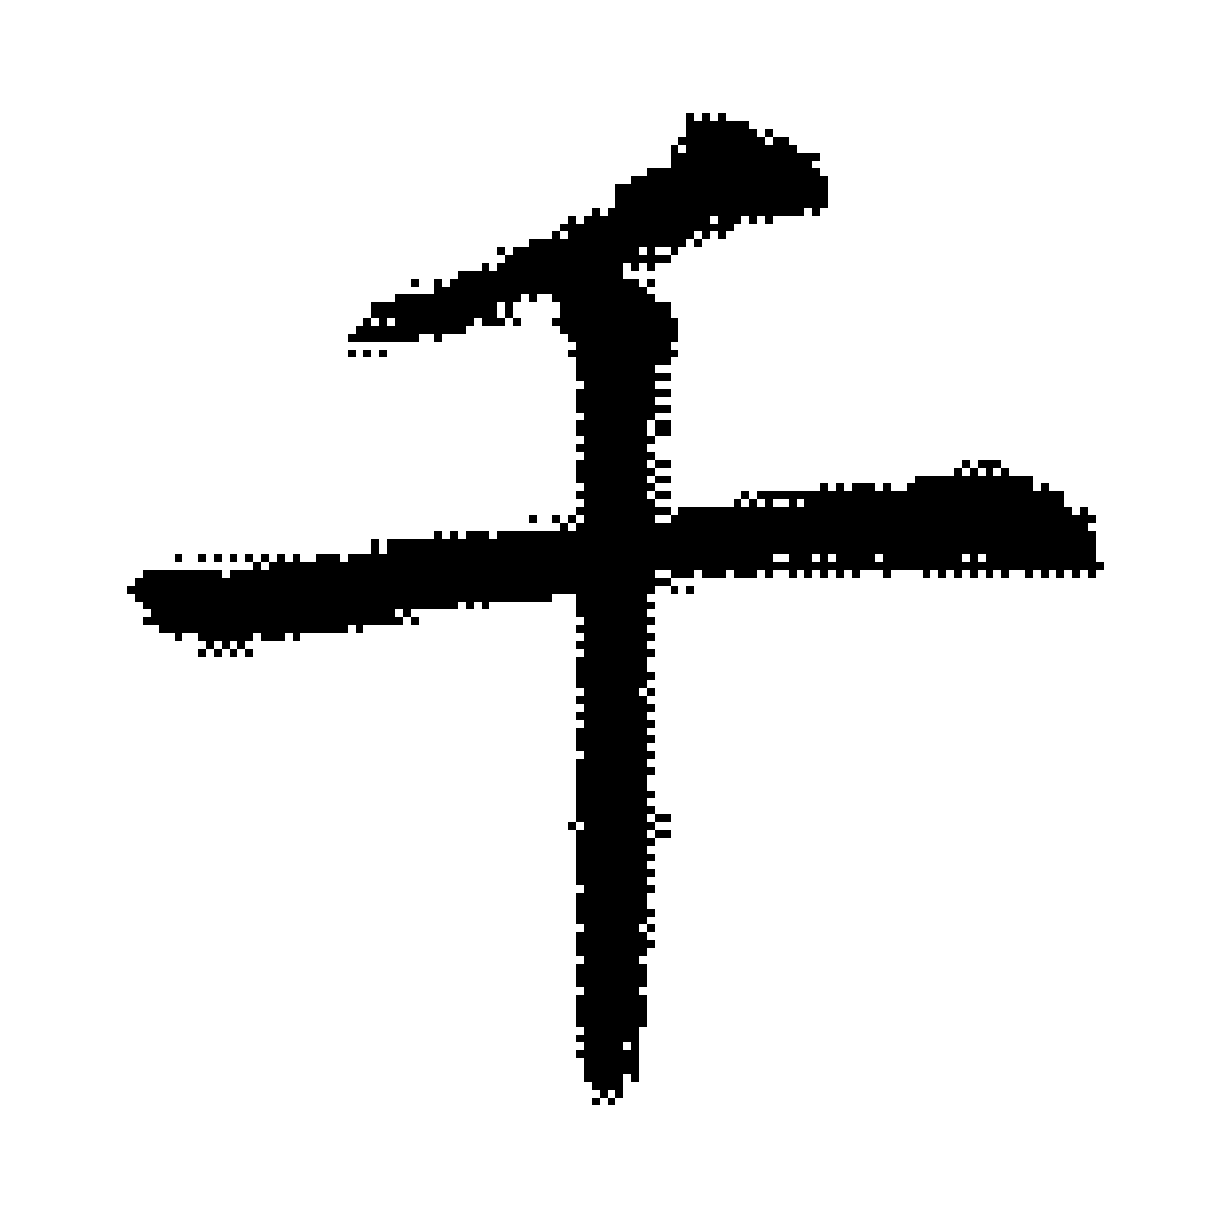
\includegraphics[width=5mm]{Nombres_et_calculs/Images/N1_chinois1000} & 
\includegraphics[width=5mm]{Nombres_et_calculs/Images/N1_chinois2} & 
\includegraphics[width=5mm]{Nombres_et_calculs/Images/N1_chinois3} \\
      Chinois & & & 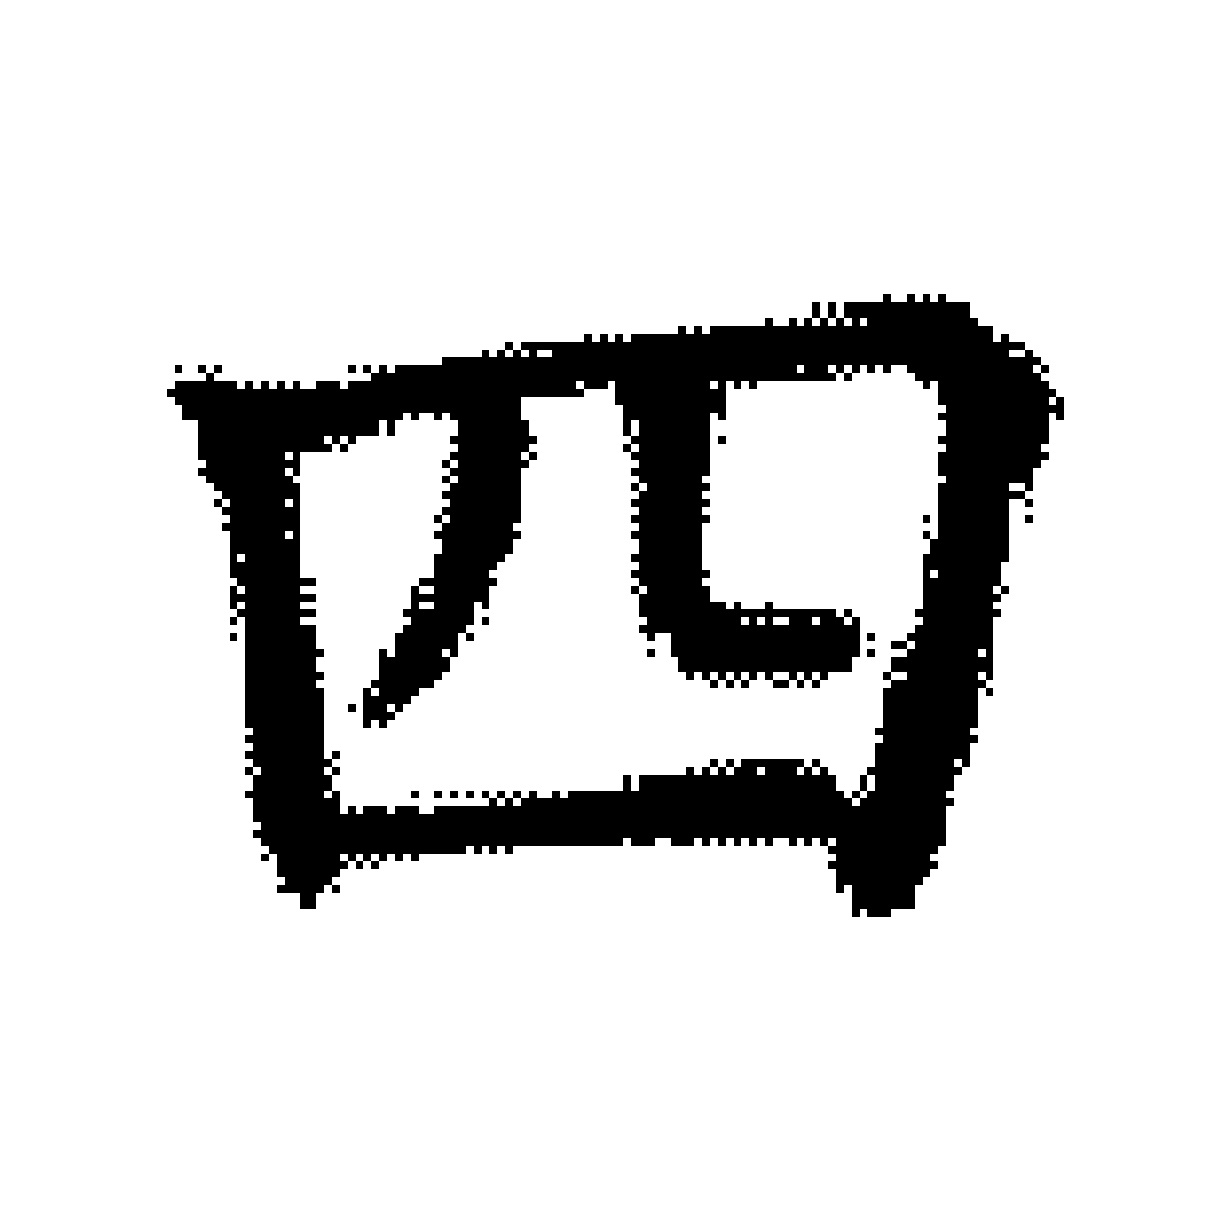
\includegraphics[width=5mm]{Nombres_et_calculs/Images/N1_chinois4} & 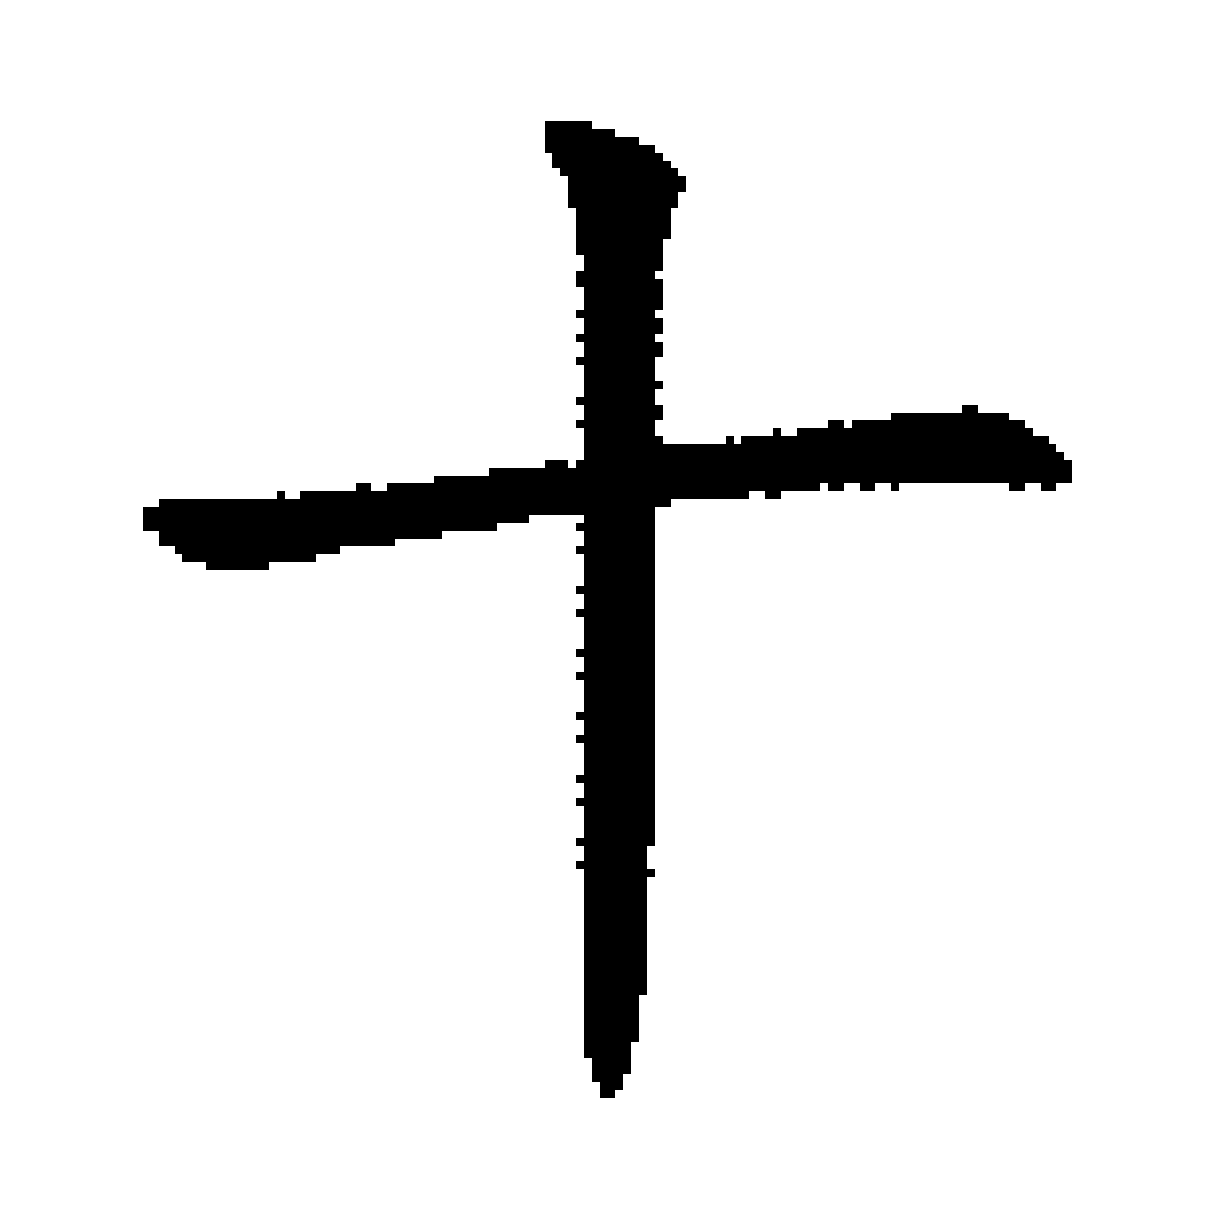
\includegraphics[width=5mm]{Nombres_et_calculs/Images/N1_chinois10} & & \\
      & & & 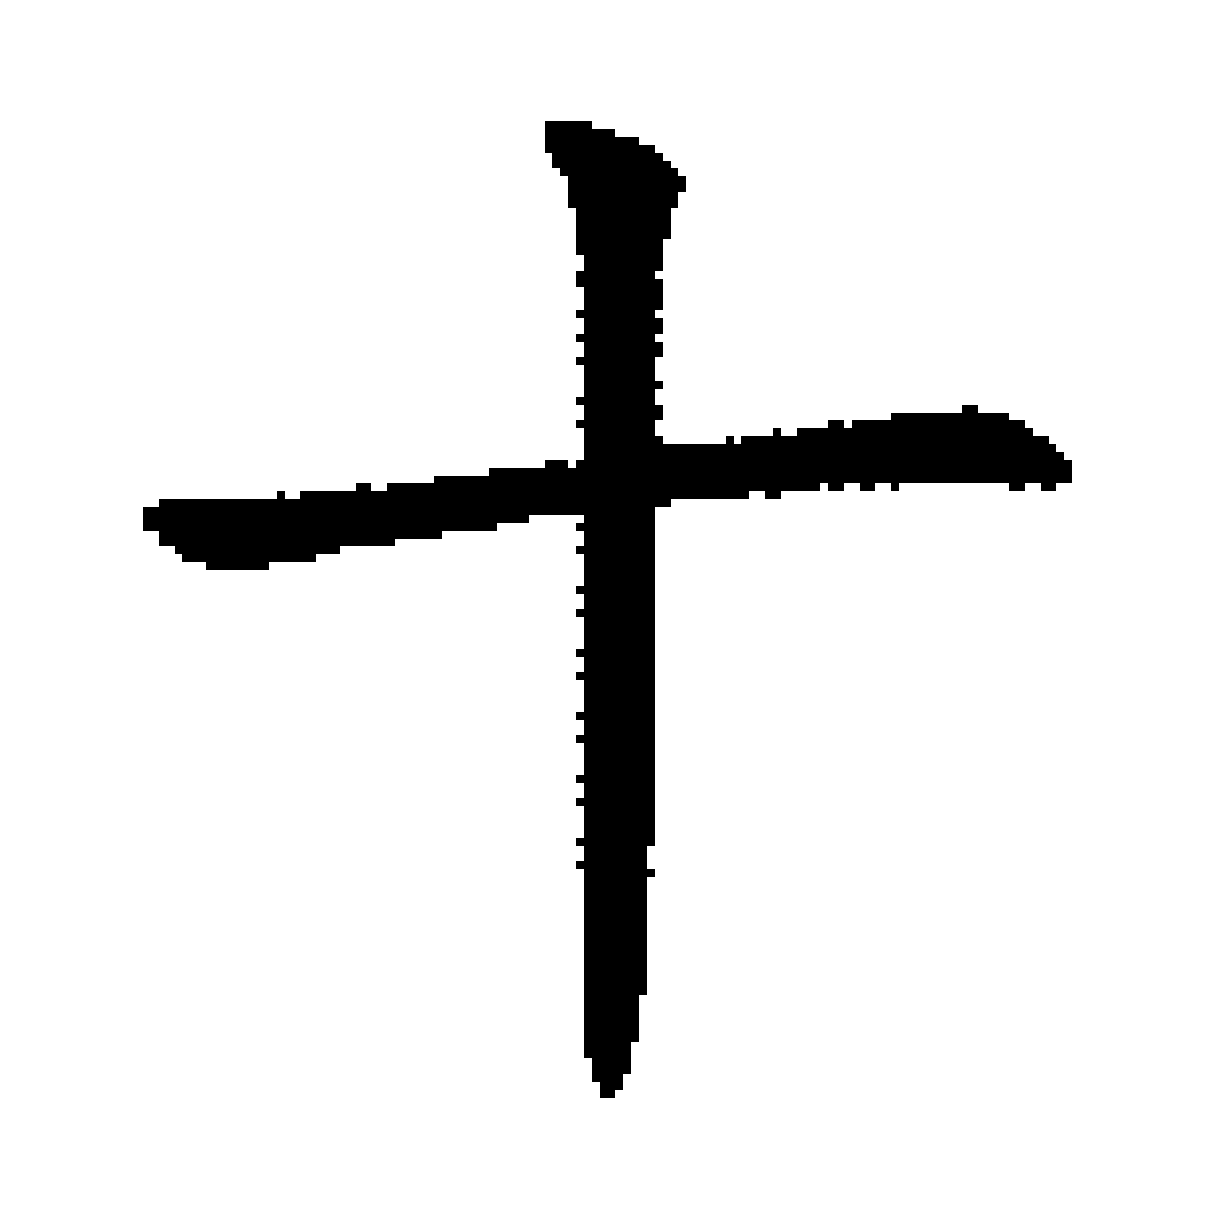
\includegraphics[width=5mm]{Nombres_et_calculs/Images/N1_chinois10}  & 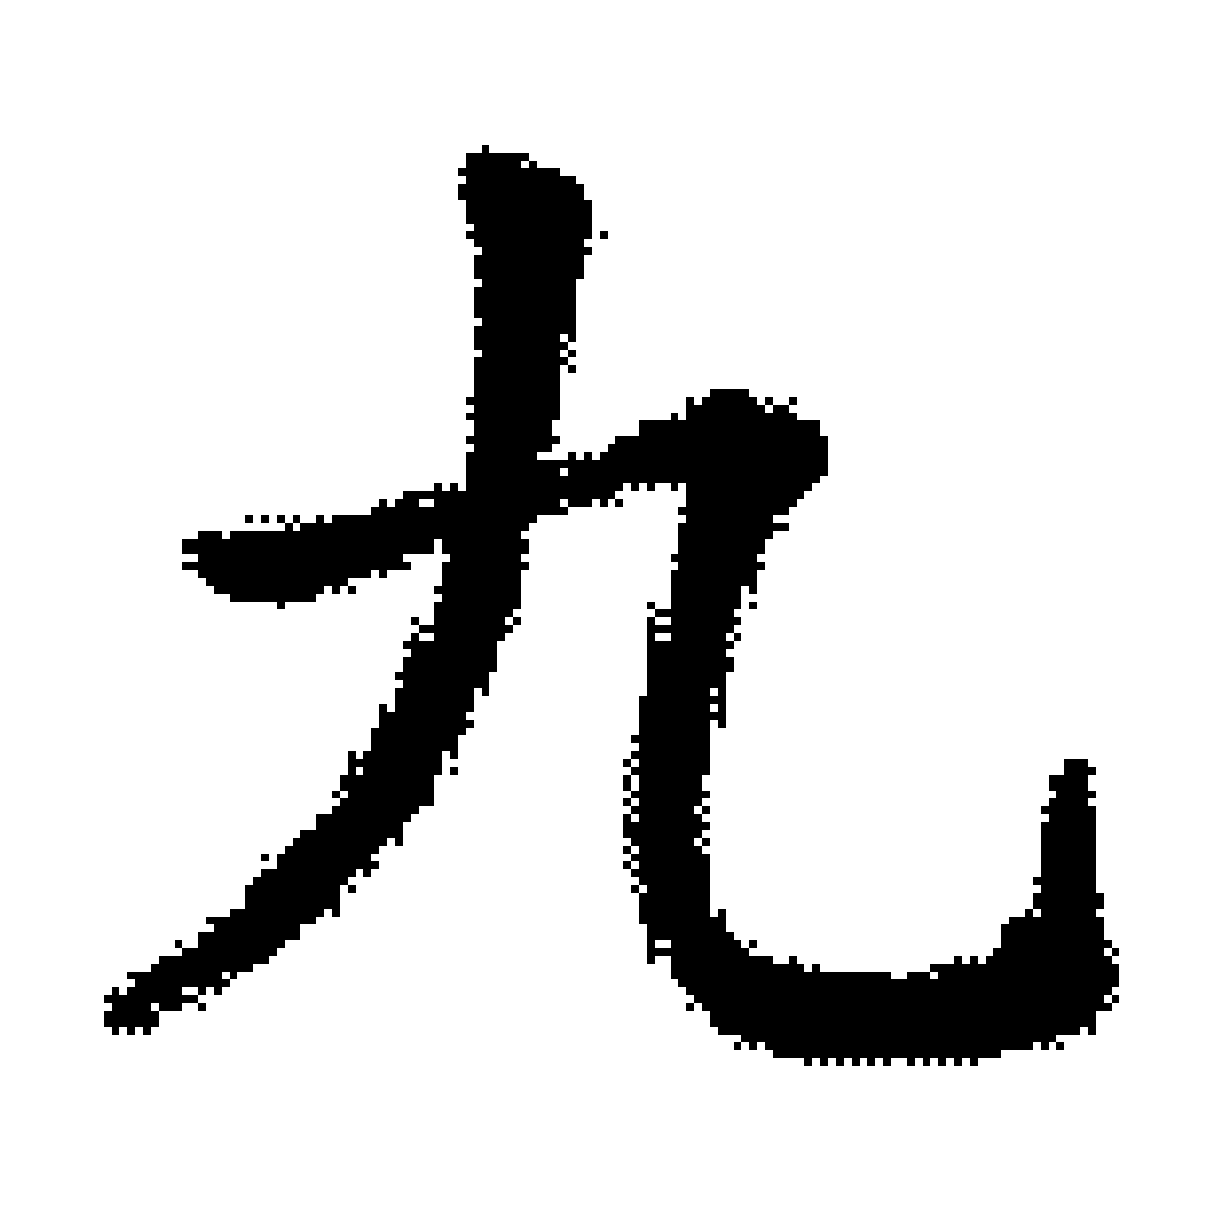
\includegraphics[width=5mm]{Nombres_et_calculs/Images/N1_chinois9} & & \\
      & & & 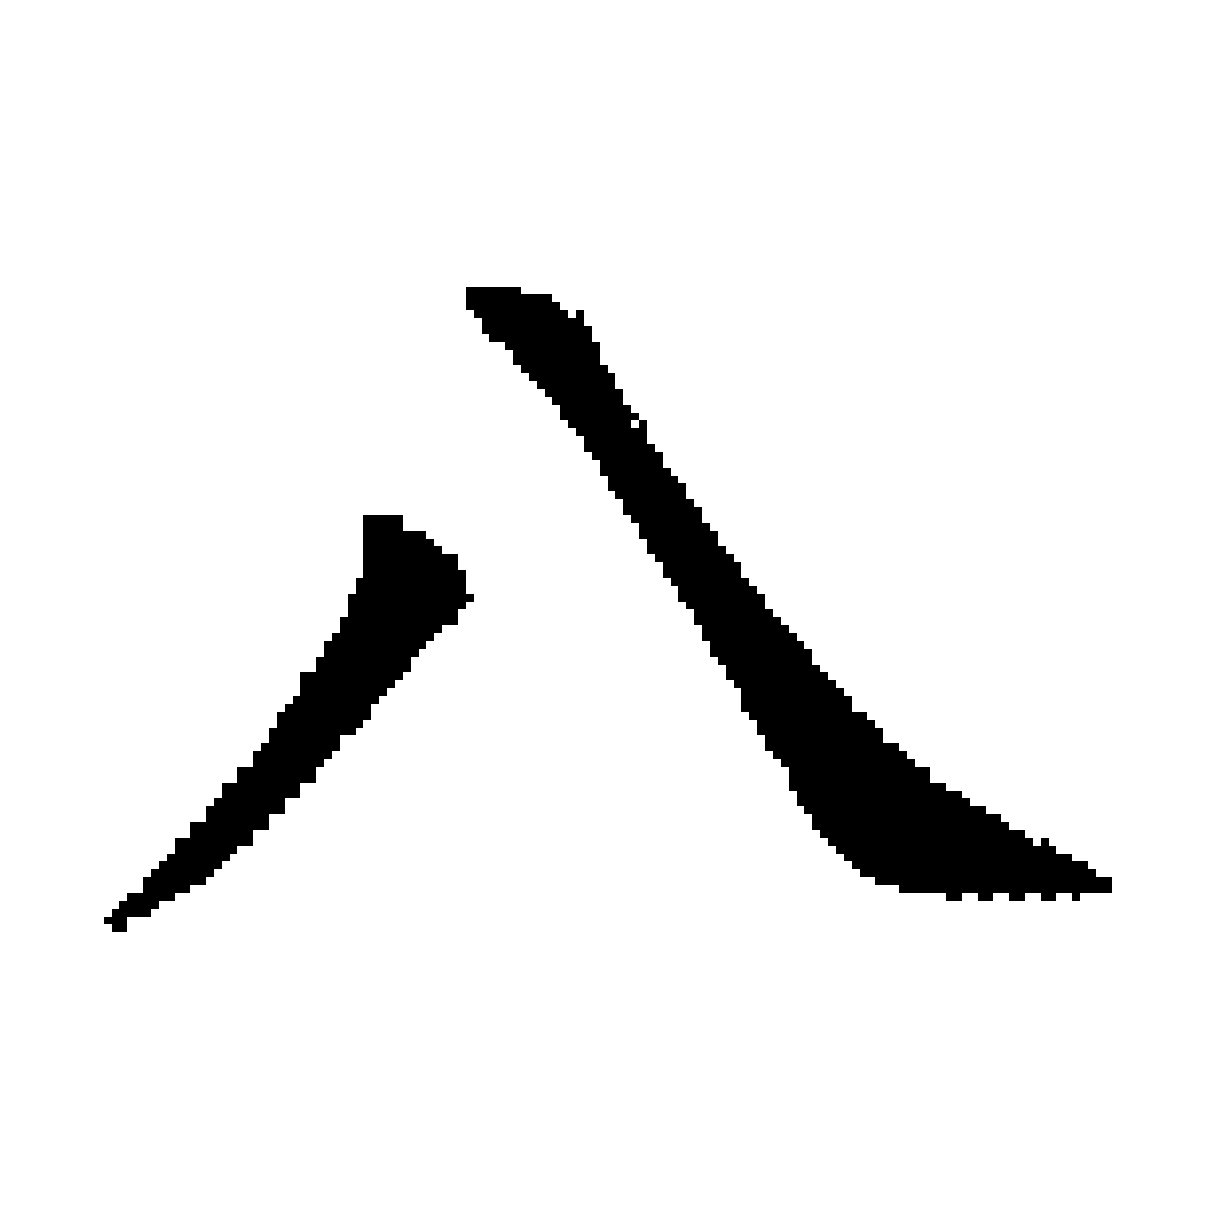
\includegraphics[width=5mm]{Nombres_et_calculs/Images/N1_chinois8} & & & \\ 
      \hline
         Maya & \large$\maya{12}$ & \large$\maya{40}$ & \large$\maya{248}$ & \large$\maya{3019}$ & \large$\maya{1002}$ & \large$\maya{1003}$ \\ [8mm]
      \hline
      Binaire & 1100 & 101000 & 11111000 & 10111100101 & 1111101010 & 1111101011 \\
      \hline
   \end{cltableau}}}
   \begin{remarque}
      la numération Maya n'utilisait pas strictement une base 20, il existait en effet une irrégularité où le passage de l'ordre 2 à l'ordre 3 nécessitait une multiplication par 18 au lieu de 20. Dans le cadre du CRPE, il est très probable que cette irrégularité ne soit pas prise en compte et c'est pour ce cas que le corrigé a été fait.
   \end{remarque}
\end{corrige}


